\documentclass[13pt]{article}

\usepackage{amsmath,amsthm,amssymb}
\usepackage{extarrows}
%\xlongequal{}

\newcommand\extrafootertext[1]{%
    \bgroup
    \renewcommand\thefootnote{\fnsymbol{footnote}}%
    \renewcommand\thempfootnote{\fnsymbol{mpfootnote}}%
    \footnotetext[0]{#1}%
    \egroup
}


% Colors
\usepackage[dvipsnames]{xcolor}

\definecolor{C0}{HTML}{1d1d1d}
\definecolor{C1}{HTML}{1e3668}
\definecolor{C2}{HTML}{199d8b}
\definecolor{C3}{HTML}{d52f4c}
\definecolor{C4}{HTML}{5ab2d6}
\definecolor{C5}{HTML}{ffb268}
\definecolor{C6}{HTML}{ff7300} % for commenting - {fire orange}dd571c
\definecolor{C7}{HTML}{777b7e} % for remarks - {steel grey}
\color{C0}
%
% fonts
\usepackage[no-math]{fontspec}

\emergencystretch=8pt
\hyphenpenalty=1000 % default 50
\tolerance=800      % default 200
%\righthyphenmin=4
%\lefthyphenmin=4

\setmainfont[
    BoldFont = Vollkorn-Bold,
    ItalicFont = Vollkorn-Italic,
    BoldItalicFont={Vollkorn-BoldItalic},
    RawFeature=+lnum,
]{Vollkorn}
\newfontfamily\myfont{Copperplate-Gothic-Bold-Regular}% not good, sad
\usepackage[scale=.78]{luatexja-fontspec}
\setmainjfont{BabelStone Han}[AutoFakeBold]

% This package simplifies the insertion of external multi-page PDF or PS doc- uments.
\usepackage{pdfpages}

% cref
\usepackage{hyperref}
\hypersetup{
    colorlinks=true,
    linkcolor=C4,
    filecolor=magenta,      
    urlcolor=cyan,
    }

\usepackage[nameinlink,noabbrev,capitalize]{cleveref}
% \crefname{ineq}{}{}
% \crefname{equation}{}{}
% \creflabelformat{ineq}{#2{\textup{(1)}}#3}
% \creflabelformat{equation}{#2\textup{(#1)}#3}

% theorem-like environment
\newtheorem{theorem}{Theorem}[section]
\newtheorem{assumption}[theorem]{Assumption}
\newtheorem{lemma}[theorem]{Lemma}
\newtheorem{corollary}[theorem]{Corollary}
\newtheorem{proposition}[theorem]{Proposition}
\newtheorem{property}[theorem]{Property}

\newtheorem{definition}[theorem]{Definition}

\theoremstyle{definition}
\newtheorem{example}[theorem]{Example}
\newtheorem{problem}[theorem]{Problem}

% framed package is great
\usepackage{framed}
\newenvironment{solution}
{\color{C2}\begin{framed}\begingroup\textbf{Solution:} }
  {\endgroup\end{framed}}

\newtheoremstyle{remark}% name of the style to be used
  {}% measure of space to leave above the theorem. E.g.: 3pt
  {}% measure of space to leave below the theorem. E.g.: 3pt
  {\color{C3}}% name of font to use in the body of the theorem
  {}% measure of space to indent
  {\color{C3}\bfseries}% name of head font
  {.}% punctuation between head and body
  { }% space after theorem head; " " = normal interword space
  {}
\theoremstyle{remark}
\newtheorem{remarkx}[theorem]{Remark}
\newenvironment{remark}
  {\pushQED{\qed}\renewcommand{\qedsymbol}{$\triangle$}\remarkx}
  {\popQED\endremarkx}
  
\newenvironment{point}
  {\O~~}
  {}

\usepackage{thmtools}
\usepackage{thm-restate}




% Page Formatting
\usepackage[
    paper=a3paper,      % b5 is optional
    inner=22mm,         % Inner margin
    outer=22mm,         % Outer margin
    bindingoffset=0mm, % Binding offset
    top=28mm,           % Top margin
    bottom=22mm,        % Bottom margin
    %showframe,         % show how the type block is set on the page
]{geometry}

\setlength{\parindent}{0em}
\setlength{\parskip}{.7em}


\usepackage{tikz}
\usepackage{graphicx}
\usepackage{enumitem}
\setlist{topsep=0pt}

\usepackage{bm}

\usepackage[font=scriptsize,labelfont=bf]{caption}
\usepackage{listings}
\lstset{basicstyle=\ttfamily,breaklines=true}
% \setlength{\parskip}{1em}
% \setlength{\parindent}{0em}
\usepackage{dsfont}
\newcommand{\bOne}{\mathds{1}}
\newcommand{\PP}{\mathbb{P}}
\newcommand{\EE}{\mathbb{E}}
\newcommand{\VV}{\mathbb{V}}
\newcommand{\CoV}{\operatorname{Co\mathbb{V}}}

% header
\usepackage{fancyhdr}
\pagestyle{fancy}
\fancyhead{}
\fancyhead[L]{\small   \bfseries Quant Review}
\fancyhead[C]{\small   \bfseries Fall 2022}
\fancyhead[R]{\small   \bfseries Zhou}





\begin{document}



\begin{center}
\title{Quant Review}
    \text{\Large{Probability and Statistics
}}
    
    {\text{Kaiwen Zhou}}


\end{center}

\tableofcontents
\newpage

\vspace{2em}

\section{Probability}
\subsection{Basic Probability Space}
\begin{point}
    \textbf{Sample Space $\Omega$:} the set of all outcomes.

    \textbf{E.g.} $\Omega$ might be the set $\Omega_{roulette}$ of 38 American roulette outcomes $\{s_1, \dots, s_{38}\} = \{1, \dots, 36, 0, 00\}$
\end{point}  

\begin{point}
    \textbf{Event:} A subset of the sample space.
    
    \textbf{E.g.} $\{2,4,\dots,36\}$ representing the "even" event 
\end{point}

\begin{point}
    \textbf{$\sigma$-algebra $\mathcal{F}$:} A $\sigma$-algebra on $\Omega$ is a collection of subsets of $\Omega$ that (a) includes the empty set; (b) is closed under complement; and (c) is closed under countable union and intersection.
    
    \textbf{E.g.} $\{0, \emptyset\}$, $2^{|\Omega|}$- the power set of $\Omega$.
\end{point}

\begin{point}
    \textbf{measurable space:} The pair $(\Omega,\mathcal{F})$ is called a measurable space.

\end{point}

\begin{point}
    \textbf{probability measure:} A probability measure on a measurable space $(\Omega,\mathcal{F})$ maps $\mathcal{F}$ into the unit interval $[0,1]$ and satisfies $\PP(\emptyset)=0$, $\PP(\Omega)=1$, and
$$p\bigl(\bigcup_{i} E_i\bigr) = \sum_{i} p_i$$
where the $E_i$ are a countable collection of pairwise disjoint events in $S$.

\end{point}

\begin{point}
    \textbf{probability space:} $(\Omega,\mathcal{F},\PP)$

\end{point}

\subsubsection{Independence}
\begin{point}
    \textbf{independent events:} Two events $A$ and $B$ are said to be independent if $\PP(A \cap B)=\PP(A) \PP(B)$. 

\end{point}

\begin{remark}\hfill

    Independence can arise in two distinct ways. Sometimes, we explicitly assume that two events are independent. For example, in tossing a coin twice, we usually assume the tosses are independent which reflects the fact that the coin has no memory of the first toss. In other instances, we derive independence by verifying that $\PP(A \cap B)=\PP(A) \PP(B)$ holds. For example, in tossing a fair die, let $A=\{2,4,6\}$ and let $B=\{1,2,3,4\}$. Hence, $A \cap B=\{2,4\}$, $\PP(A\cap B)=2 / 6=\PP(A) \PP(B)=(1 / 2) \times(2 / 3)$ and so $A$ and $B$ are independent. In this case, we didn't assume that $A$ and $B$ are independent it just turned out that they are. In fact, the independence is less than obvious here. Intuitively, $A$ and $B$ are independent because knowing $A$ does not change the probability of $B$. We shall make this point more precise when we discuss conditional probability.

Suppose that $A$ and $B$ are disjoint events, each with positive probability. Can they be independent? No. This follows since $\PP(A) \PP(B)>0$ yet $\PP(A B)=\PP(\emptyset)=0$. Except in this special case, there is no way to judge independence by looking a the sets in a Venn diagram. The events $A_{1}, \ldots, A_{k}$ are defined to be independent if, for any $I \subset$ $\{1, \ldots, k\}$ we have that

\end{remark}

\begin{corollary}
$$
\PP\left(\cap_{i \in I} A_{i}\right)=\prod_{i \in I} \PP\left(A_{i}\right) .
$$

For example, three events $A_{1}, A_{2}$ and $A_{3}$ are independent if they satisfy

$$
\begin{aligned}
\PP\left(A_{1} A_{2}\right)  =\PP\left(A_{1}\right) \PP\left(A_{2}\right), \quad
\PP\left(A_{1} A_{3}\right) & =\PP\left(A_{1}\right) \PP\left(A_{3}\right), \quad
\PP\left(A_{2} A_{3}\right) =\PP\left(A_{2}\right) \PP\left(A_{3}\right), \\
\PP\left(A_{1} A_{2} A_{3}\right) & =\PP\left(A_{1}\right) \PP\left(A_{2}\right) \PP\left(A_{3}\right) .
\end{aligned}
$$
\end{corollary}

\subsubsection{Conditional Probability}
\begin{point}
    \textbf{conditional probability:} 
    
    \textbf{E.g.} the \textbf{conditional probability} of event A, given that event B has occurred, is written $\PP(A\mid B)$, and by definition equals
$$\PP(A\mid B)=\frac{\PP(A\cap B)}{\PP(B)}$$
\end{point}

\begin{remark}\hfill
\begin{enumerate}[label=(\arabic*)]
    \item One interpretation is that this is a rule for updating our probability of $A$ once we know that $B$ has occurred. Another interpretation is that, upon repetitions, $\PP(A \mid B)$ is the fraction of times $A$ occurs among those in which $B$ occurs.
    \item In our die example, consider the event $A=\{1\}$ so that $\PP(A)=1 / 6$. Suppose we are now told that the outcome is odd. Then, we would no longer use $\PP(A)=1 / 6$ but rather $\PP(A \mid B)=\PP(A \cap B) / \PP(B)=(1 / 6) /(3 / 6)=1 / 3$ where $B=\{1,3,5\}$.
    \item In general it is not the case that $\PP(A \mid B)=\PP(B \mid A)$. People get this confused all the time. For example, the probability of spots given you have measles is 1 but the probability that you have measles given that you have spots is not 1 . In this case, the difference between $\PP(A \mid B)$ and $\PP(B \mid A)$ is obvious. But there are cases where it is less obvious.
    \item Suppose that $A$ and $B$ are independent events. Then,

$$
\PP(A \mid B)=\frac{\PP(A\cap  B)}{\PP(B)}=\frac{\PP(A) \PP(B)}{\PP(B)}=\PP(A) .
$$

Thus, independence implies that $\PP(A \mid B)=\PP(A)$ and that $\PP(B \mid A)=\PP(B)$. So another interpretation of independence is that knowing $B$ doesn't change the probability of $A$.
\end{enumerate}
\end{remark}

\subsubsection{Bayes' Theorem}
Bayes' theorem is a simple theorem that allows us to update probabilities in light of new information. First, we need a preliminary result.

\begin{theorem}\textbf{(The Law of Total Probability)} Let $A_{1}, \ldots, A_{k}$ be a partition of $S$. Then, for any event $B, \PP(B)=\sum_{i=1}^{k} \PP\left(B \mid A_{i}\right) \PP\left(A_{i}\right)$.
\end{theorem}

\begin{solution} Define $C_{j}=B \cap A_{j}$ and note that $C_{1}, \ldots, C_{k}$ are disjoint and that $B=\cup_{j=1}^{k} C_{j}$. Hence,

$$
\PP(B)=\sum_{j} \PP\left(C_{j}\right)=\sum_{j} \PP\left(B \cap A_{j}\right)=\sum_{j} \PP\left(B \mid A_{j}\right) \PP\left(A_{j}\right)
$$

since $\PP\left(B A_{j}\right)=\PP\left(B \mid A_{j}\right) \PP\left(A_{j}\right)$ from the definition of conditional probability.
\end{solution}


\begin{theorem}\textbf{(Bayes' Theorem)} Let $A_{1}, \ldots, A_{k}$ be a partition of $S$ such that $\PP\left(A_{i}\right)>0$ for each $i$. Let $B$ be an event such that $\PP(B)>0$. Then, for each $i=1, \ldots, k$,
\[
\PP\left(A_{i} \mid B\right)=\frac{\PP\left(B \mid A_{i}\right) \PP\left(A_{i}\right)}{\sum_{j} \PP\left(B \mid A_{j}\right) \PP\left(A_{j}\right)} .
\]
\end{theorem}
\begin{solution}We apply the definition of conditional probability twice, followed by the law of total probability:
\[
\PP\left(A_{i} \mid B\right)=\frac{\PP\left(A_{i} \cap B\right)}{\PP(B)}\xlongequal{\text{conditional prob}}\frac{\PP\left(B \mid A_{i}\right) \PP\left(A_{i}\right)}{\PP(B)}=\frac{\PP\left(B \mid A_{i}\right) \PP\left(A_{i}\right)}{\sum_{j} \PP\left(B \mid A_{j}\right) \PP\left(A_{j}\right)}.
\]
\end{solution}
\begin{remark}
    In Bayesian inference, $\PP\left(A_{i}\right)$ is called the "prior probability of $A_{i}$ " and $\PP\left(A_{i} \mid B\right)$ is called the "posterior probability of $A_{i}$." To some extent, Bayes' theorem is an expression of how probabilities are updated as information is acquired. 
\end{remark}

\subsubsection{Random Variables}

\begin{point}
    \textbf{random variable:} a \textbf{random variable} $X$ is a function that maps $\Omega$ into the real numbers $\mathbb{R}$, where $\Omega$ is the sample space of a probability space $(\Omega,\mathcal{F},\PP)$.

\end{point}

\begin{remark}\hfill
    \begin{enumerate}
        \item Flip a coin ten times. Each outcome $s$ consists of a sequence of 10 coin tosses, for example, $s=H H T H H T H H T T$. Let $X(s)$ be the number of heads in the sequence $s$. Thus, if $s=HHTHHTHHTT$ then $X(s)=6$. Note that $S$ has $2^{10}$ elements while $X$ can only take values in $\{0, \ldots, 10\}$.

    \end{enumerate}
\end{remark}

\begin{definition}\textbf{(Distribution of R.V.)}
Given a random variable $X$ and a subset $A$ of the real line, define
\[
F_{X}(A)=P(X \in A)=P\left(X^{-1}(A)\right)=P(\{s \in S ; X(s) \in A\}) .
\]
Then $F_{X}$ is called the distribution of $X$.
\end{definition}
\begin{remark}Flip a coin twice and let $X$ be the number of heads. This random variable can only take values 0,1 or 2 . Clearly, $P(X=0)=$ $P(\{T T\})=1 / 4, P(X=1)=P(\{H T, T H\})=1 / 2$ and $P(X=2)=$ $P(\{H H\})=1 / 4$. We can compute other probabilities as well. For example, $P(.3 \leq X \leq 17)=P(X=1)+P(X=2)=3 / 4$. It might seem strange to compute the probability that $X$ falls in the interval $[.3,17]$ but this serves to emphasize that we can compute that probability for any subset $A$ of the real line.
\end{remark}

\begin{point}
    \textbf{cumulative distribution function (cdf):} 
    \[F_X(x)=\PP(X\leq x)\]

\end{point}

\subsection{Discrete Random Variables}
$X$ is discrete if it takes countably many values (the sample space $\Omega$ is finite or countably infinite). If $X$ is discrete, we define its probability mass function by

\begin{point}
    \textbf{probability mass function:} If (a) the sample space $\Omega$ is finite or countably infinite; and (b) the $\sigma$-algebra is the power set of $\Omega$, then the probability measure is a \textbf{probability mass function p} that assigns a value $\PP(\omega)$ to each $\omega\in\Omega$, where $\sum_{\omega\in\Omega}\PP(\omega)=1$.

    If (a) is true but not (b), then there are one or more probability mass functions that are compatible with the probability measure.

    \textbf{E.g.} suppose $\Omega$ consists of the six outcomes of the throw of a single die, and $S=\{\emptyset,\{1\},\{2,3,4,5,6\},\Omega\}$. A probability measure that assigns $\frac{1}{6}$ to the event $\{1\}$ and $\frac{5}{6}$ to the event $\{2,3,4,5,6\}$ is compatible with the usual mass function that assigns $\frac{1}{6}$ to each outcome. It is also compatible with a mass function that assigns $\frac{1}{6}$ to each of $1,2,3,4;$ assigns $\frac{1}{3}$ to $5$; and zero to $6$.
\end{point}

The CDF of $X$ is
\[
F_{X}(x)=P(X \leq x)=\sum_{s \leq x} f(s) .
\]
\begin{remark}
    Suppose that $X$ is a discrete random variable and that $P(X=0)=P(X=2)=1 / 4$ and $P(X=1)=1 / 2$. Thus, $f(0)=$ $f(2)=1 / 4$ and $f(1)=1 / 2$. The cdf is given by
\[
F(x)= \begin{cases}0 & \text { if } x<0 \\ \frac{1}{4} & \text { if } 0 \leq x<1 \\ \frac{3}{4} & \text { if } 1 \leq x<2 \\ 1 & \text { if } x \geq 2\end{cases}
\]
\end{remark}
\subsubsection{Point Mass Distribution}
$X$ has a point mass distribution at $a$, written $X \sim \delta_{a}$, if
\[
F(x)= \begin{cases}0 & x<a \\ 1 & x \geq a .\end{cases}
\]

\subsubsection{Uniform Distribution}Let $k>1$ be a given integer. Suppose that $X$ has probability mass function given by
\[
pmf(x)= \begin{cases}\frac{1}{k} & \text { for } x=1, \ldots, k \\ 0 & \text { otherwise. }\end{cases}
\]

We say that $X$ has a uniform distribution on $\{1, \ldots, k\}$.

\subsubsection{Bernoulli Distribution}
Let $X$ represent a coin flip. Then $P(X=1)=p$ and $P(X=0)=1-p$ for some $p \in[0,1] . X$ has a Bernoulli distribution written $X \sim \operatorname{Bernoulli}(p)$.

\subsubsection{Binomial Distribution} Suppose we have a coin which falls heads with probability $p$ for some $0 \leq p \leq 1$. Flip the coin $n$ times and let $X$ be the number of heads. Assume that the tosses are independent. Let $pmf(x)=P(X=x)$ be the mass function. It can be shown that

$$
pmf(x)= \begin{cases}\binom{n}{x} p^{x}(1-p)^{n-x} & \text { for } x=0, \ldots, n \\
0 & \text { otherwise. }\end{cases}
$$

A random variable with such mass function is called a Binomial random variable and we write $X \sim \operatorname{Binom}(n, p)$ to say that $X$ has this distribution.

\begin{remark}\textbf{(Warning!)}
    Let us take this opportunity to prevent some confusion. $X$ is a random variable; $x$ denotes a particular value of the random variable; $n$ and $p$ are "parameters", that is, fixed real numbers. Parameters are not random. (At least not yet.) 
    
    The parameter $p$ is often unknown and must be estimated from data; that's what statistical inference is all about. In most statistical models, there are random variables and parameters: don't confuse them.
\end{remark} 

\subsubsection{Geometric Distribution}$X$ has a geometric distribution with parameter $p \in(0,1)$, written $X \sim \operatorname{Geom}(p)$, if
$$
P(X=k)=p(1-p)^{k-1}, \quad k \geq 1 .
$$
We have that
$$
\sum_{k=1}^{\infty} P(X=k)=p \sum_{k=0}^{\infty}(1-p)^{k}=\frac{p}{1-(1-p)}=1 .
$$

Think of $X$ as the number of flips needed until the first heads on a coin with $P(Heads)=p$.

\subsubsection{Poisson Distribution}
$X$ has a Poisson distribution with parameter $\lambda$, written $X \sim \operatorname{Poisson}(\lambda)$ if
$$
pmf(k)=e^{-\lambda} \frac{\lambda^{k}}{k !} \quad k \geq 0 .
$$
Note that
$$
\sum_{k=0}^{\infty} f(k)=e^{-\lambda} \sum_{k=0}^{\infty} \frac{\lambda^{k}}{k !}=e^{-\lambda} e^{\lambda}=1 .
$$

\subsubsection{Bivariate Distributions}
Given a pair of discrete random variables $X$ and $Y$, define the joint mass function by $f(x, y)=P(X=x$ and $Y=y)$. From now on, we write $P(X=x$ and $Y=y)$ as $P(X=x, Y=y)$. We write $f$ as $f_{X, Y}$ when we want to be more explicit.

\begin{remark}
    \textbf{(Example)} Suppose a coin is biased and has probability $2 / 3$ of falling heads. Toss the coin twice. Let $X=0$ if the first toss is tails and $X=1$ if the first toss is heads. Define $Y$ analogously for the second toss. Then, $f(0,0)=P(X=0, Y=0)=1 / 9, f(1,0)=P(X=1, Y=0)=2 / 9$, $f(0,1)=P(X=0, Y=1)=2 / 9, f(1,1)=P(X=1, Y=1)=4 / 9$.

\begin{center}
\begin{tabular}{l|ll|l}
 & $Y=0$ & $Y=1$ &  \\
\hline
$\mathrm{X}=0$ & $1 / 9$ & $2 / 9$ & $1 / 3$ \\
$\mathrm{X}=1$ & $2 / 9$ & $4 / 9$ & $1 / 3$ \\
\hline
 & $1 / 3$ & $1 / 3$ & 1 \\
\hline
\end{tabular}
\end{center}
\end{remark}
 
\subsubsection{Marginal Distributions}
If $(X, Y)$ have joint distribution with mass function $f_{X, Y}$, then the marginal mass function for $X$ is defined by $f_{X}(x)=P(X=x)=\sum_{y} P(X=$ $x, Y=y)=\sum_{y} f(x, y)$ and the marginal mass function for $Y$ is defined by $f_{Y}(y)=P(Y=y)=\sum_{x} P(X=x, Y=y)=\sum_{x} f(x, y)$.
\begin{remark}
    \textbf{(Example)} Suppose that $f_{X, Y}$ is given in the table that follows. The marginal distribution for $X$ corresponds to the row totals and the marginal distribution for $Y$ corresponds to the columns totals. For example, $f_{X}(0)=3 / 10$ and $f_{X}(1)=7 / 10$.

\begin{center}
\begin{tabular}{l|ll|l}
 & $Y=0$ & $Y=1$ &  \\
\hline
$\mathrm{X}=0$ & $1 / 10$ & $2 / 10$ & $3 / 10$ \\
$\mathrm{X}=1$ & $3 / 10$ & $4 / 10$ & $7 / 10$ \\
\hline
 & $4 / 10$ & $6 / 10$ & 1 \\
\hline
\end{tabular}
\end{center}
\end{remark}

\subsection{Continuous Random Variables}

A random variable $X$ is said to be continuous, or more accurately, is said to have a continuous distribution, if there is a function $f$ such that (i) $f_{X}(x) \geq 0$, (ii) $\int f_{X}(x) d x=1$ and (iii) $P(X \in A)=\int_{A} f_{X}(x) d x$. We call $f_{X}$ the probability density function (pdf) for $X$. We use the convention that $\int f(x) d x$ with no limits of integration is to be interpreted to mean $\int_{-\infty}^{\infty} f(x) d x$. The cdf is $F_{X}(x)=\int_{-\infty}^{x} f(s) d s$. 

\begin{point}
    \textbf{probability density function (pdf):} $\frac{d}{dx}F_X(x)=f_X(x)$.

    \textbf{E.g.} The most widely used probability distributions include the uniform distribution $F(x)=x$ where $0\leq x\leq 1$; and the normal distribution $\text{pdf}(x)=\frac{1}{\sqrt{2\pi}}\exp(-x^2/2)$.
\end{point} 

\begin{property}\textbf{(Two useful properties of CDF)}
\begin{enumerate}[label=(\alph*)]
    \item $P(X=x)=F\left(x^{+}\right)-F\left(x^{-}\right)$.
    \item $F\left(x_{2}\right)-F\left(x_{1}\right)=P\left(X \leq x_{2}\right)-P\left(X \leq x_{1}\right).$
\end{enumerate}
\end{property}

\begin{remark}
    \textbf{(Warning!)} Continuous random variables can lead to confusion. First, note that if $X$ is continuous then $P(X=x)=0$ for every $x$ ! Don't try to think of $f_X(x)$ as $P(X=x)$. This only holds for discrete random variables. One recovers probabilities from a pdf by integrating it. 
    
    A pdf can be bigger than 1 (unlike a mass function). For example, if $f(x)=5$ for $x \in[0,1 / 5]$ and 0 otherwise, then $f(x) \geq 0$ and $\int f(x) d x=1$ so this is a well-defined pdf even though $f(x)=5$ in some places. In fact, a pdf can be unbounded. For example, if $f(x)=(2 / 3) x^{-1 / 3}$ for $0<x<1$ and $f(x)=0$ otherwise, then check that $\int f(x) d x=1$ even though $f$ is not bounded.
\end{remark}

It is also useful to define the inverse cdf or quantile function. 
\begin{definition}\textbf{(Quantile Function)} Suppose that $F$ is strictly increasing and continuous. Then, given a $q \in[0,1]$, there is a real number $x$ such that $F(x)=q$. We write $x=F^{-1}(q)$. For example, $F^{-1}(1 / 4)$ is the number $x$ such that $P(X \leq x)=1 / 4$. More generally, define 
\[
F^{-1}(q)=\inf \{x: F(x) \leq q\}.
\]
This allows us define the inverse cdf even in the discrete case. We call $F^{-1}(1 / 4)$ the first quartile, $F^{-1}(1 / 2)$ the median (or second quartile) and $F^{-1}(3 / 4)$ the third quartile.
\end{definition}

\begin{remark}\hfill
    \begin{enumerate}
        \item \textbf{(pdf should be well-defined)} Suppose that $X$ has pdf
\[
f(x)= \begin{cases}c & \text { for } x \in[a, b] \\ 0 & \text { otherwise. }\end{cases}
\]
Here $a<b$ are real numbers and $c$ is constant. Since we require the pdf to be  well-defined, i.e. $\int f(x) d x=1$, it follows that $c=1 /(b-a)$. 

A random variable with this distribution is said to have a Uniform (a,b) distribution. Each value between $a$ and $b$ us equally likely. We write $X \sim \operatorname{Unif}(a, b)$. The median is $(a+b) / 2$. The first quartile is $(3 / 4) a+(1 / 4) b$.
\item \textbf{(ill-defined pdf)} Let
\[
f(x)= \begin{cases}0 & \text { for } x<0 \\ \frac{c}{(1+x)} & \text { otherwise }\end{cases}
\]

This is not a pdf since $\int f(x) d x=c \int_{1}^{\infty} d u / u=c \log (\infty)=\infty$
\item \textbf{(From CDF to pdf)} Suppose that
\[
F(x)= \begin{cases}0 & \text { if } x<0 \\ \frac{x}{1+x} & \text { if } x \geq 0\end{cases}
\]
Then, by differentiating $F$ we see that
\[
f(x)=F^{\prime}(x)= \begin{cases}0 & \text { if } x<0 \\ \frac{1}{(1+x)^{2}} & \text { if } x \geq 0\end{cases}
\]
    \end{enumerate}
\end{remark}

\subsubsection{Uniform Distribution} $X$ has a Uniform $(a, b)$ distribution where $a<b$, written $X \sim \operatorname{Uniform}(a, b)$, if
\[
f(x)= \begin{cases}\frac{1}{b-a} & \text { for } x \in[a, b] \\ 0 & \text { otherwise }\end{cases}, \quad F(x)= \begin{cases}0 & x<a \\ \frac{x-a}{b-a} & x \in[a, b] \\ 1 & x>b .\end{cases} 
\]

\begin{remark}
    The definition of a "uniform distribution" is that the density function is constant for all $x$ (or $x, y$) within the support region. So one must have
    \[
    f_{X}(x) = \frac{1}{A}, \quad \text{or} \quad f_{X,Y}(x,y) = \frac{1}{A}
    \]
    where $A$ is the area of either the square or the circle.

\textbf{The same formula will hold for the density function of a "uniform distribution" on any geometric region.}

E.g. Let $(X, Y)$ be uniform on the unit square. Then, we must have  $f_{X,Y}(x,y) = \frac{1}{A}$. Hence, by simple integration, we can get
$$
f(x, y)= \begin{cases}1 & \text { if } 0 \leq x \leq 1,0 \leq y \leq 1 \\ 0 & \text { otherwise. }\end{cases}
$$
\end{remark}
\subsubsection{Normal (Gaussian) Distribution} $X$ has a Normal, or Gaussian distribution with parameters $\mu$ and $\sigma$, $\mu \in \mathbb{R}$ and $\sigma>0$ denoted by $X \sim N\left(\mu, \sigma^{2}\right)$, if
\[
f(x)=\frac{1}{\sigma \sqrt{2 \pi}} \exp \left\{-\frac{1}{2}\left(\frac{x-\mu}{\sigma}\right)^{2}\right\}, \quad x \in \mathbb{R}
\]
We say that $X$ has a \textbf{standard Normal distribution} if $\mu=0$ and $\sigma=1$. The cdf is $\Phi(x)=\int_{-\infty}^{x} f(s) d s$ which does not have a closed form expression. 
\begin{remark}\hfill
    \begin{enumerate}
        \item If $X \sim N\left(\mu, \sigma^{2}\right)$ and $Z=(X-\mu) / \sigma$ then $Z \sim N(0,1)$.
        \item If $Z \sim N(0,1)$ and $X=\mu+\sigma Z$ then $X \sim N\left(\mu, \sigma^{2}\right)$
        \item If $X \sim N\left(\mu, \sigma^{2}\right)$ then $\EE[e^X]=e^{\mu+\frac{1}{2}\sigma^2}$.
    \end{enumerate}
\end{remark}

\subsubsection{Exponential Distribution} $X$ has an exponential distribution with parameter $\beta$, denoted by $X \sim \operatorname{Exp}(\beta)$, if
\[
f(x)=\frac{1}{\beta} e^{-x / \beta}, \quad x>0
\]
where $\beta>0$.

\subsubsection{Gamma Distribution} For $\alpha>0$, the Gamma function is defined by $\Gamma(\alpha)=\int_{0}^{\infty} y^{\alpha-1} e^{-y} d y . X$ has an Gamma distribution with parameters $\alpha$ and $\beta$, denoted by $X \sim \operatorname{Gamma}(\alpha, \beta)$, if

$$
f(x)=\frac{1}{\beta^{\alpha} \Gamma(\alpha)} x^{\alpha-1} e^{-x / \beta}, \quad x>0
$$

where $\alpha, \beta>0$.

\subsubsection{Bivariate Distributions}
\begin{definition}\textbf{(joint density function)}
    In the continuous case, we call a function $f(x, y)$ a joint pdf for the random variables $(X, Y)$ if 
\begin{enumerate}[label=(\roman*)]
    \item $f(x, y) \geq 0$ for all $(x, y)$,
    \item $\int_{-\infty}^{\infty} \int_{-\infty}^{\infty} f(x, y) d x d y=1$
    \item $\forall A \subset \mathbb{R} \times \mathbb{R}, P((X, Y) \in A)=\iint_{A} f(x, y) d x d y$.
\end{enumerate}
\end{definition}

\begin{definition}\textbf{(joint CDF)}
    We define the joint cdf as 
    \[F_{X, Y}(x, y)=P(X \leq x, Y \leq y).
    \]
\end{definition}
\begin{remark}\hfill 
    \begin{enumerate}
        \item \textbf{(Warning!)} There are two types of bivariate distributions. (i) The \textbf{Domain of $X, Y$ is Rectangles.} These rectangles can be infinite, such as the whole plane. The rectangle case is easy because the range of one variable does not depend on the range of the other variable. (ii) The \textbf{Domain of $X, Y$ is NOT Rectangle.} The non-rectangle case is hard because the range of one variable does depend on the range of the other variable. 
        \item \textbf{(Domain of $X, Y$ is Rectangles case)} Let $(X, Y)$ be uniform on the unit square. Hence,
$$
f(x, y)= \begin{cases}1 & \text { if } 0 \leq x \leq 1,0 \leq y \leq 1 \\ 0 & \text { otherwise. }\end{cases}
$$
Find $P(X<1 / 2, Y<1 / 2)$. 
\begin{solution}
The event $A=\{X<1 / 2, Y<1 / 2\}$ corresponds to a subset of the unit square. Integrating $f$ over this subset corresponds, in this case, to computing the area of the set $A$ which is $1 / 4$. That is,
\[
P(X<1 / 2, Y<1 / 2) = \int_0^{\frac{1}{2}}\int_0^{\frac{1}{2}}f(x, y) dxdy = \frac{1}{4}.
\]
So, $P(X<$ $1 / 2, Y<1 / 2)=1 / 4$.
\end{solution}
\item \textbf{(Domain of $X, Y$ is Non-rectangle case)} Let $(X, Y)$ have density
$$
f(x, y)= \begin{cases}c x^{2} y & \text { if } x^{2} \leq y \leq 1 \\ 0 & \text { otherwise. }\end{cases}
$$
Find $P(X \geq Y)$.
\begin{solution}
Note first that $-1 \leq x \leq 1$. Now let us find the value of $c$. The trick here is to be careful about the range of integration. We pick one variable, $x$ say, and let it range over its values. Then, for each fixed value of $x$, we let $y$ vary over its range which is $x^{2} \leq y \leq 1$. Thus,
$$
\begin{aligned}
\iint f(x, y) d y d x & =c \int_{-1}^{1} \int_{x^{2}}^{1} x^{2} y d y d x \\
& =c \int_{-1}^{1} x^{2}\left[\int_{x^{2}}^{1} y d y\right] d x \\
& =c \int_{-1}^{1} x^{2} \frac{1-x^{4}}{2} d x \\
& =\frac{4 c}{21} .
\end{aligned}
$$
Hence, $c=21 / 4$. 

Now let us compute $P(X \geq Y)$. This corresponds to the set $A=\left\{(x, y) ; 0 \leq x \leq 1, x^{2} \leq y \leq x\right\}$. (You can see this by drawing a diagram.) So,
$$
\begin{aligned}
P(X \geq Y) & =\frac{21}{4} \int_{0}^{1} \int_{x^{2}}^{x} x^{2} y d y d x \\
& =\frac{21}{4} \int_{0}^{1} x^{2}\left[\int_{x^{2}}^{x} y d y\right] d x \\
& =\frac{21}{4} \int_{0}^{1} x^{2} \frac{x^{2}-x^{4}}{2} d x \\
& =\frac{3}{20} .
\end{aligned}
$$
\end{solution}
    \end{enumerate}
\end{remark}

 
\subsubsection{Marginal Distributions}
\begin{definition}\textbf{(Marginal Density Function)} If $(X, Y)$ have joint distribution with joint density function $f_{X, Y}$, then \begin{enumerate}[label=(\alph*)]
    \item The marginal density function for $X$ is defined by $f_{X}(x)=\int f(x, y) d y$,
    \item The marginal density function for $Y$ is defined by $f_{Y}(y)=\int f(x, y) d x$.
\end{enumerate}
\end{definition}

\begin{remark}\hfill 
\begin{enumerate}
    \item \textbf{(Warning!)}Again, we need to distinguish rectangle and non-rectangle cases. The integral $f_{X}(x)=\int f(x, y) d y$ is easy in the rectangle case. It is harder in the non-rectangle case. 
    \item \textbf{(Domain of $X, Y$ is Rectangle case)} Suppose that
$$
f_{X, Y}(x, y)=e^{-(x+y)}
$$
for $x, y \geq 0$. Then $f_{X}(x)=e^{-x} \int_{0}^{\infty} e^{-y} d y=e^{-x}$.
\item \textbf{(Domain of $X, Y$ is Non-rectangle case)} Let $(X, Y)$ have density
$$
f(x, y)= \begin{cases}c x^{2} y & \text { if } x^{2} \leq y \leq 1 \\ 0 & \text { otherwise. }\end{cases}
$$
Find the marginal density function for $X$.
\begin{solution}
We know from the above notes, $c=21 / 4$. 

Let us find the marginal for $X$. In this case, $x^{2} \leq y \leq 1$, then we have
$$
\begin{aligned}
f_{X}(x) & =\int f(x, y) d y \\
& =\frac{21}{4} x^{2} \int_{x^{2}}^{1} y d y=\frac{21}{8} x^{2}\left(1-x^{4}\right)
\end{aligned}
$$
for $-1 \leq x \leq 1$ and $f_{X}(x)=0$ otherwise.
\end{solution}
\end{enumerate}
\end{remark}

\subsubsection{Independent Random Variables}
Two random variables $X$ and $Y$ are independent if, for every $A$ and $B$, $P(X \in A, Y \in B)=P(X \in A) P(Y \in B)$. In this case we write $X \amalg Y$. 

In principle, to check whether $X$ and $Y$ are independent we need to check this equation for all subsets $A$ and $B$. Fortunately, we have the following result which we state for continuous random variables though it is true for discrete random variables too.

\begin{theorem} Let $X$ and $Y$ have joint pdf $f_{X, Y}$. Then $X \amalg Y$ if and only if 
\[
f_{X, Y}(x, y)=f_{X}(x) f_{Y}(y)
\]for all values $x$ and $y.$
\end{theorem}
\begin{remark}\hfill
    \begin{enumerate}
        \item Let $X$ and $Y$ be such that $P(X=0, Y=0)=$ $P(X=0, Y=1)=P(X=1, Y=0)=P(X=1, Y=1)=1 / 4$. Then, $f_{X}(0)=f_{X}(1)=1 / 2$ and $f_{Y}(0)=f_{Y}(1)=1 / 2 . X$ and $Y$ are independent because $f_{X}(0) f_{Y}(0)=f(0,0), f_{X}(0) f_{Y}(1)=f(0,1), f_{X}(1) f_{Y}(0)=f(1,0)$, $f_{X}(1) f_{Y}(1)=f(1,1)$.

\begin{center}
\begin{tabular}{l|ll|l}
 & $Y=0$ & $Y=1$ &  \\
\hline
$\mathrm{X}=0$ & $1 / 4$ & $1 / 4$ & $1 / 2$ \\
$\mathrm{X}=1$ & $1 / 4$ & $1 / 4$ & $1 / 2$ \\
\hline
 & $1 / 2$ & $1 / 2$ & 1 \\
\hline
\end{tabular}
\end{center}

Suppose instead that $P(X=0, Y=0)=P(X=1, Y=1)=1 / 2$ and $P(X=0, Y=1)=P(X=1, Y=0)=0$. These are not independent because $f_{X}(0) f_{Y}(1)=(1 / 2)(1 / 2)=1 / 4$ yet $f(0,1)=0$.

\begin{center}
\begin{tabular}{l|ll|l}
 & $Y=0$ & $Y=1$ &  \\
\hline
$\mathrm{X}=0$ & $1 / 2$ & 0 & $1 / 2$ \\
$\mathrm{X}=1$ & 0 & $1 / 2$ & $1 / 2$ \\
\hline
 & $1 / 2$ & $1 / 2$ & 1 \\
\hline
\end{tabular}
\end{center}
\item Suppose that $X$ and $Y$ are independent and both have the same density
$$
f(x)= \begin{cases}2 x & \text { if } 0 \leq x \leq 1 \\ 0 & \text { otherwise. }\end{cases}
$$
Let us find $P(X+Y \leq 1)$.
\begin{solution}
    This turns out to be a "non-rectangle" calculation. 
    
    Since $X,Y$ are independent, the joint density is
$$
f_{X,Y}(x, y)=f_{X}(x) f_{Y}(y)= \begin{cases}4 x y & \text { if } 0 \leq x \leq 1, \quad 0 \leq y \leq 1 \\ 0 & \text { otherwise. }\end{cases}
$$
Here it is if you are interested:
$$
\begin{aligned}
{\color{C3}P(X+Y \leq 1)} & ={\color{C3}\iint_{x+y \leq 1} f_{X,Y}(x, y) d y d x} \\
& ={\color{C3}4 \int_{0}^{1} x\left[\int_{0}^{1-x} y d y\right] d x} \\
& =4 \int_{0}^{1} x \frac{(1-x)^{2}}{2} d x=\frac{1}{6} .
\end{aligned}
$$
\end{solution}
    \end{enumerate}
\end{remark}



\begin{theorem} \textbf{(A useful result)} Suppose that the range (domain) of $X$ and $Y$ is a (possibly infinite) rectangle. If 
\[
f_{X, Y}(x, y)=g(x) h(y)
\]
for some functions $g$ and $h$ then $X$ and $Y$ are independent.
\end{theorem} 
\begin{solution}
    The proof is simple. We have
    \begin{align*}
    f_X(x)\cdot f_Y(y) &= \int g(x)h(y) dy\cdot \int g(x)h(y) dx\\
    &= g(x)h(y)\int h(y) dy\cdot \int g(x) dx\\
    &= g(x)h(y)\iint h(y)g(x) dxdy\\
    &=g(x)h(y)\cdot \iint f_{X, Y}(x, y) dxdy\\
    &=g(x)h(y)
    \end{align*}
\end{solution}
\begin{remark}Let $X$ and $Y$ have density
$$
f_{X,Y}(x, y)= \begin{cases}2 e^{-(x+2 y)} & \text { if } x>0 \text { and } y>0 \\ 0 & \text { otherwise. }\end{cases}
$$
The range of $X$ and $Y$ is the rectangle $(0, \infty) \times(0, \infty)$. 

We can write $f_{X,Y}(x, y)=$ $g(x) h(y)$ where $g(x)=2 e^{-x}$ and $h(y)=e^{-2 y}$. Thus, $X \amalg Y$.
\end{remark} 
\subsubsection{Conditional Distributions}
\begin{definition}\textbf{(conditional mass function)}
    If $X$ and $Y$ are discrete, then we can compute the conditional distribution of $X$ given that we have observed $Y=y$. Specifically, $P(X=x \mid Y=y)=$ $P(X=x, Y=y) / P(Y=y)$. This leads us to define the conditional mass function
$$
f_{X \mid Y}(x \mid y)=P(X=x \mid Y=y)=\frac{P(X=x, Y=y)}{P(Y=y)}=\frac{f_{X, Y}(x, y)}{f_{Y}(y)} .
$$
Similarly, the mass function for $Y$ given $X$ is defined by $f_{Y \mid X}(y \mid x)=\frac{f_{X, Y}(x, y)}{f_{X}(x)}.$
\end{definition}

\begin{definition}\textbf{(conditional density function)}For continuous distributions we use the same definitions. 
$$
f_{X \mid Y}(x \mid y)=\frac{f_{X, Y}(x, y)}{f_{Y}(y)} .
$$
The interpretation differs: in the discrete case, $f_{X \mid Y}(x \mid y)$ is $P(X=x \mid Y=y)$ but in the continuous case, we must integrate $f_{X \mid Y}(x \mid y)$ to yield probability statements:
$$
P(X \in A \mid Y=y)=\int_{A} f_{X \mid Y}(x \mid y) d x .
$$
A useful way of thinking about this is to think of $A$ as $[x, x+h]$ where $h$ is a small positive.
\end{definition}

\begin{corollary}\textbf{(A useful result)}
        From the definition of the conditional density, we see that 
        \[f_{X, Y}(x, y)=f_{X \mid Y}(x \mid y) f_{Y}(y)=f_{Y \mid X}(y \mid x) f_{X}(x).
        \]
\end{corollary}
\begin{remark}\hfill 
    \begin{enumerate}
        \item \textbf{(Warning!)} We are treading in deep water here. When we compute $P(X \in A \mid Y=y)$ in the continuous case we are actually conditioning on a set of probability 0 ! We avoided problems by defining things in terms of the pdf. The fact that this leads to a well-defined theory is proved in more advanced courses. We simply take it as a definition. 
        \item \textbf{(Domain of $X, Y$ is Rectangle case)} Let $X$ and $Y$ have a uniform distribution on the unit square. Verify that $f_{X \mid Y}(x \mid y)=1$ for $0 \leq x \leq 1$ and 0 otherwise. Thus, given $Y=y, X$ is Uniform $(0,1)$. We can write this as $X \mid Y=y \sim \operatorname{Unif}(0,1)$.
        \begin{solution}
            Since $(X, Y)$ be uniform on the unit square. Then, we must have  
            $$
            f_{X,Y}(x, y)= \begin{cases}1 & \text { if } 0 \leq x \leq 1,0 \leq y \leq 1 \\ 0 & \text { otherwise. }\end{cases}
            $$
            By simple calculation, we get the marginal density of $Y$ to be 
            $
            f_{Y}(y)= \int_0^1 f_{X,Y}(x, y) dx = 1
            $.
            Therefore, we have
            \[
            f_{X \mid Y}(x \mid y)=\frac{f_{X, Y}(x, y)}{f_{Y}(y)}=\frac{1}{1} =1 \Longrightarrow \PP(X\le t \mid Y=y) = \int_0^t 1 dx =t
            \]
            This suggests that given $Y=y, X$ is Uniform $(0,1)$, i.e. $X \mid Y=y \sim \operatorname{Unif}(0,1)$.
        \end{solution}  
        \item \textbf{(Domain of $X, Y$ is Rectangle case)} Let
$$
f(x, y)= \begin{cases}x+y & \text { if } 0 \leq x \leq 1,0 \leq y \leq 1 \\ 0 & \text { otherwise. }\end{cases}
$$
Find $P\left(X<\frac{1}{4} \mid Y=\frac{1}{3}\right)$.
\begin{solution}
Earlier we saw that $f_{Y}(y)=y+(1 / 2)$. Hence,
$$
f_{X \mid Y}(x \mid y)=\frac{f_{X, Y}(x, y)}{f_{Y}(y)}=\frac{x+y}{y+\frac{1}{2}} .
$$
So
$$
\begin{aligned}
P\left(X<\frac{1}{4} \mid Y=\frac{1}{3}\right) & =\int_{0}^{1 / 4} f_{X \mid Y}\left(x \mid \frac{1}{3}\right) d x \\
& =\int_{0}^{1 / 4} \frac{x+\frac{1}{3}}{\frac{1}{3}+\frac{1}{2}} d x \\
& =\frac{\frac{1}{32}+\frac{1}{3}}{\frac{1}{3}+\frac{1}{2}} \\
& =\frac{14}{32} .
\end{aligned}
$$
\end{solution}
\item \textbf{(Domain of $X, Y$ is Non-rectangle case)} Suppose that $X \sim \operatorname{Unif}(0,1)$. After obtaining a value of $X$ we generate $Y \mid X=x \sim \operatorname{Unif}(x, 1)$. What is the marginal distribution of $Y$ ? 

\begin{solution}Since $Y \mid X=x \sim \operatorname{Unif}(x, 1)$, we must have $x\le y \le 1$. Then, we obtain
$$
f_{X}(x)= \begin{cases}1 & \text { if } 0 \leq x \leq 1 \\ 0 & \text { otherwise }\end{cases}, \quad \text{and} \quad f_{Y \mid X}(y \mid x)= \begin{cases}\frac{1}{1-x} & \text { if } 0<x<y<1 \\ 0 & \text { otherwise }\end{cases}
$$
So,
$$
f_{X, Y}(x, y)=f_{Y \mid X}(y \mid x) f_{X}(x)= \begin{cases}\frac{1}{1-x} & \text { if } 0<x<y<1 \\ 0 & \text { otherwise. }\end{cases}
$$
Computing the marginal for $Y$ is a non-rectangle problem:
$$
f_{Y}(y)=\int_{0}^{y} f_{X, Y}(x, y) d x=\int_{0}^{y} \frac{d x}{1-x}=-\log (1-y)
$$
for $0<y<1$.
\end{solution}
\item \textbf{(Domain of $X, Y$ is Non-rectangle case)} Let $(X, Y)$ have density
$$
f(x, y)= \begin{cases}c x^{2} y & \text { if } x^{2} \leq y \leq 1 \\ 0 & \text { otherwise. }\end{cases}
$$
Compute $P(Y \geq 3 / 4 \mid X=1 / 2)$.
\begin{solution}
    We know from the above notes, $c=21 / 4$. 
    
Now let's find $f_{Y \mid X}(y \mid x)$. When $X=x, y$ must satisfy $x^{2} \leq y \leq 1$. Earlier, we saw that $f_{X}(x)=(21 / 8) x^{2}\left(1-x^{4}\right)$. Hence, for $x^{2} \leq y \leq 1$,
$$
f_{Y \mid X}(y \mid x)=\frac{f_{X,Y}(x, y)}{f_{X}(x)}=\frac{\frac{21}{4} x^{2} y}{\frac{21}{8} x^{2}\left(1-x^{4}\right)}=\frac{2 y}{1-x^{4}}
$$
Now let us compute $P(Y \geq 3 / 4 \mid X=1 / 2)$. This can be computed by first noting that $f_{Y \mid X}(y \mid 1 / 2)=32 y / 15$. Thus, {\color{C3}(Don't forget that we must have $x^{2} \leq y \leq 1$ !)}
$$
P(Y \geq 3 / 4 \mid X=1 / 2)=\int_{\max\{3 / 4, x^2\}}^{1} f_{Y \mid X}(y \mid 1 / 2) d y=\int_{3 / 4}^{1} f_{Y \mid X}(y \mid 1 / 2) d y=\int_{3 / 4}^{1} \frac{32 y}{15} d y=\frac{7}{15}
$$
\end{solution}
    \end{enumerate}
\end{remark}

\subsubsection{Multivariate Distributions and i.i.d Samples}
\begin{point}
    \textbf{Random Vector:}Let $X=\left(X_{1}, \ldots, X_{n}\right)$ where $X_{1}, \ldots, X_{n}$ are random variables. We call $X$ a random vector. 
\end{point}

\begin{point}
    \textbf{Independence:} Let $f\left(x_{1}, \ldots, x_{n}\right)$ denote the pdf. It is possible to define their marginals, conditionals etc. much the same way as in the bivariate case. We say that $X_{1}, \ldots, X_{n}$ are independent if, for every $A_{1}, \ldots, A_{n}$,
$$
P\left(X_{1} \in A_{1}, \ldots, X_{n} \in A_{n}\right)=\prod_{i=1}^{n} P\left(X_{i} \in A_{i}\right) .
$$
It suffices to check that $f\left(x_{1}, \ldots, x_{n}\right)=\prod_{i=1}^{n} f_{X_{i}}\left(x_{i}\right)$. 
\end{point}


\begin{point}
    \textbf{i.i.d:} If $X_{1}, \ldots, X_{n}$ are independent and each has the same marginal distribution with density $f$, we say that $X_{1}, \ldots, X_{n}$ are i.i.d. (independent and identically distributed).
\end{point}

\begin{point}
    \textbf{i.i.d. samples:} We shall write this as $X_{1}, \ldots X_{n} \sim f$ or, in terms of the cdf, $X_{1}, \ldots X_{n} \sim F$. This means that $X_{1}, \ldots, X_{n}$ are independent draws from the same distribution. We also call $X_{1}, \ldots, X_{n}$ a random sample from $F$.
\end{point}

Much of statistical theory and practice begins with i.i.d. observations and we shall study this case in detail when we discuss statistics.

\begin{remark}\hfill

    Suppose that the lifetime $X$ of a light bulb is a random variable with density
$$
f_{X}(x)= \begin{cases}e^{-x} & \text { if } x>0 \\ 0 & \text { otherwise }\end{cases}
$$
Suppose we have $n$ light bulbs. Assuming that their failure times are independent, what is the joint density of their lifetimes $X_{1}, \ldots, X_{n}$. 
\begin{solution}The answer is $f\left(x_{1}, \ldots, x_{n}\right)=\prod_{i} f\left(x_{i}\right)$, hence,
$$
f\left(x_{1}, \ldots, x_{n}\right)= \begin{cases}e^{-\sum_{i=1}^{n} x_{i}} & \text { if } x_{i}>0, i=1, \ldots, n \\ 0 & \text { otherwise. }\end{cases}
$$
\end{solution}
\end{remark} 

\subsubsection{Transformations of Random Variables}
Suppose that $X$ is a random variable with $\operatorname{pdf} f_{X}$ and $\operatorname{cdf} F_{X}$. Let $Y=r(X)$ be a function of $X$, for example, $Y=X^{2}$ or $Y=e^{X}$. What are the pdf and cdf of $Y$ ? 

This question pops up in many places. We call $Y=r(X)$ a transformation of $X$. 

\begin{theorem}\textbf{(Discrete Case)} In the discrete case, the answer is easy. The mass function of $Y$ is given by
$$
f_{Y}(y)=P(Y=y)=P(r(X)=y)=P(\{x ; r(x)=y\})=P\left(X \in r^{-1}(y)\right)
$$
\end{theorem}

\begin{remark}Suppose that $f_{X}(-1)=P(X=-1)=1 / 4, f_{X}(0)=$ $P(X=0)=1 / 2$ and $f_{X}(1)=P(X=1)=1 / 4$. 

Let $Y=X^{2}$. Then, $P(Y=$ $0)=P(X=0)=1 / 2$ and $P(Y=1)=P(X=1)+P(X=-1)=1 / 2$. Hence, $f_{Y}(0)=1 / 2$ and $f_{Y}(1)=1 / 2$.
\end{remark}

\begin{theorem}Here is a suggestion: figure out the answer in terms of the cdf then find the pdf. 

Thus, we calculate
$$
F_{Y}(y)=P(Y \leq y)=P(r(X) \leq y)=P(\{x ; r(x) \leq y\})=\int_{A_{y}} f_{X}(x) d x
$$
where $A_{y}=\{x ; r(x) \leq y\}$. The only hard part is finding $A_{y}$.
\end{theorem}

\begin{remark}\hfill
    \begin{enumerate}
        \item 
There are two cases. If $r$ is monotone increasing or decreasing, the problem is easy since we can take the inverse of $r$. Otherwise, it is tricky. 
\item \textbf{($r$ is monotone increasing or decreasing)} Let $f_{X}(x)=e^{-x}$ for $x>0$. Then $F_{X}(x)=\int_{0}^{x} f_{X}(s) d s=$ $1-e^{-x}$. Let $Y=r(X)=\log X \longrightarrow r$ is monotone increasing. Then
$$
F_{Y}(y)=P(Y \leq y)=P(\log X \leq y)=P\left(X \leq e^{y}\right)=F_{X}\left(e^{y}\right)=1-e^{-e^{y}} .
$$
Therefore, $f_{Y}(y)=F_Y'(y)=e^{y} e^{-e^{y}}$ for $y \in \mathbb{R}$.

\textbf{Warning!} It is tempting to transform the densities instead of the random variables. This is wrong. In the last example, $\log f_{X}(x)=-x \neq f_{Y}$.
\item \begin{theorem}
    \textbf{(A useful result)} When $r$ is strictly monotone increasing or strictly monotone decreasing then $r$ has an inverse $s=r^{-1}$ and in this case one can show that
$$
f_{Y}(y)=f_{X}(s(y))\left|\frac{d s(y)}{d y}\right|
$$
\end{theorem}
    \end{enumerate}
\end{remark}

\begin{problem}
    \textbf{(when $r$ is not monotone 1)} Let $X \sim \operatorname{Unif}(-1,1)$. Find the pdf of $Y=X^{2}$. Find $f_Y(y)$.
\end{problem}

\begin{solution}
    
    First, we see that
$$
f_{X}(x)= \begin{cases}\frac{1}{2} & \text { if }-1<x<1 \\ 0 & \text { otherwise. }\end{cases}
$$
Clearly, $Y$ can only take values in $(0,1)$. For any $y \in(0,1)$,
$$
F_{Y}(y)  =P(Y \leq y)=P\left(X^{2} \leq y\right)
=P(-\sqrt{y} \leq X \leq \sqrt{y})
=\int_{-\sqrt{y}}^{\sqrt{y}} f_{X}(x) d x=\sqrt{y}.
$$
So, $A_{y}=[-\sqrt{y}, \sqrt{y}]$ for $0<y<1$ and $A_{y}=\emptyset$ otherwise. Now, $f_{Y}(y)=F^{\prime}(y)$ so
$$
f_{Y}(y)= \begin{cases}\frac{1}{2 \sqrt{y}} & \text { if } 0<y<1 \\ 0 & \text { otherwise. }\end{cases}
$$
\end{solution}

\begin{problem}
    \textbf{(when $r$ is not monotone 2)} Let $X \sim \operatorname{Unif}(-1,3)$. Find the pdf of $Y=X^{2}$. Find $f_Y(y)$.
\end{problem}
\begin{solution}
    First, we see that
$$
f_{X}(x)= \begin{cases}\frac{1}{4} & \text { if }-1<x<3 \\ 0 & \text { otherwise }\end{cases}
$$
First, we note that $Y$ can only take values in $(0,9)$. Then, we have
\[
F(Y\le y) = F(X^2\le y) = F(-\sqrt{y}\le X\le \sqrt{y}) = \int_{\max\{-\sqrt{y},-1\}}^{\min\{\sqrt{y},3\}} f_X(x)dx
\]
Since $Y$ can only take values in $(0,9)$, we must have $\min\{\sqrt{y},3\}=\sqrt{y}$. 
\begin{enumerate}[label=(\roman*)]
    \item If $-\sqrt{y}<-1$, i.e. $1\le y < 9$, then we have 
    \[
    F(Y\le y) = \int_{-1}^{\sqrt{y}} f_X(x)dx = \frac{\sqrt{y}}{4}+\frac{1}{4}
    \]
    \item If $-\sqrt{y}\ge-1$, i.e. $0\le y < 1$, then we have 
    \[
    F(Y\le y) = \int_{-\sqrt{y}}^{\sqrt{y}} f_X(x)dx = \frac{\sqrt{y}}{2}
    \]
\end{enumerate}
Differentiating $F$ we get
$$
f_{Y}(y)= \begin{cases}\frac{1}{4 \sqrt{y}} & \text { if } 0<y<1 \\ \frac{1}{8 \sqrt{y}} & \text { if } 1<y<9 \\ 0 & \text { otherwise. }\end{cases}
$$
\end{solution}

\subsubsection{The Probability Integral Transform}
The last section discussed transformations in general. Here we study one special transformation. 

\begin{problem}\textbf{($F_{X}(X)$ has a Unif $(0,1)$)} Let $X$ has a continuous, strictly increasing cdf $F_{X}$. Define $Y=F_X(X)$. That is, we draw a random variable $X$ whose cdf is $F_X$, then we evaluate the cdf at the randomly selected point. What distribution does $Y$ have? 
\end{problem}
\begin{solution}
    Since $0 \leq F_X(x) \leq 1$ for all $x$, we see that $Y$ can only take values between 0 and 1. Given a point $y$, let $x=F_{X}^{-1}(y)$ i.e. find $x$ such that $F_{X}(x)=y$. Such a point exists and is unique. Then, we have
    \[
    Y=F_X(X)\le y \Longleftrightarrow X\le F^{-1}_X(y) = x
    \]
    That is, $Y$ is less than $y$ if and only if $X$ is less than $x$. Thus, 
    \[
    F_{Y}(y)=P(Y \leq y)=P(X \leq x)=F_{X}(x)=y.
    \]
    So we have shown that $F_{Y}(y)=y$. This is the cdf for a $\operatorname{Unif}(0,1)$ random variable. We have proved that $F_{X}(X)$ has a Unif $(0,1)$ distribution.
\end{solution}
\begin{proposition}\textbf{(all purpose random number generator)} Assume we have a way to generate random numbers from a Unif $(0,1)$ distribution. (There are lots of algorithms for doing this). Let $X$ be a random variable with continuous, strictly increasing cdf $F_{X}$. How can we generate a random $X$ having distribution $F_{X}$? 
\end{proposition}
\begin{solution}
    {\color{C3} We can do this by drawing (sampling) $Y \sim \operatorname{Unif}(0,1)$. Then define $X=H(Y)$ where $H=F_{X}^{-1}$. We claim that $X$ has the right distribution.}
    
    To see this, we compute the CDF of $X$ and verify that it is $F_{X}$. Recall that since $Y$ has a $\operatorname{Unif}(0,1)$ distribution that $P(Y \leq y)=F_{Y}(y)=y$ for $0<y<1$. Now
$$
P(X \leq x)=P(H(Y) \leq x)=P\left(F_{X}^{-1}(Y) \leq x\right)=P\left(Y \leq F_{X}(x)\right)=F_{X}(x)
$$
as required.
\end{solution}

\subsubsection{Functions of Several Random Variables}
In some cases we are interested in transformation of several random variables. For example, if $X$ and $Y$ are given random variables, we might want to know the distribution of $X / Y$ or $X+Y$. 

In principle one proceeds as before. We start with the joint pdf $f_{X, Y}(x, y)$. Let $Z=r(X, Y)$ be the function of interest. Then we compute the CDF of $Z$ :
$$
F_{Z}(z)=P(Z \leq z)=\iint_{A_{z}} f(x, y) d x d y
$$
where $A_{z}=\{(x, y) ; r(x, y) \leq z\}$. Finally, we get $f_{Z}$ be differentiating $F_{Z}$. 
\begin{remark}\hfill
    \begin{enumerate}
        \item Finding $A_{z}$ and doing the integral can be hard in some cases, but conceptually the idea is the same as before. Some cases of special interest are summation and averaging. Suppose that $X_{1}, \ldots, X_{n}$ are random variables and let $Z=r\left(X_{1}, \ldots, X_{n}\right)=n^{-1} \sum_{i=1}^{n} X_{i}$. How do we find the distribution of $Z$ ? We deal with this in Chapter 4.
        \item 
    \end{enumerate}
\end{remark}


\begin{point}
    \textbf{characteristic function:} If $X$ is a random variable, then its characteristic function $\varphi_X(t)$ is
$$\varphi_X(t)=\int e^{itx}dF_X(x)=\int e^{itx}f_X(x)dx$$
where $F_X(x)$ and $f_X(x)$ are respectively the cdf and pdf of the probability distribution and $i$ is the imaginary unit.

    Thus the characteristic function is the Fourier transform of the pdf. If the pdf is symmetric about zero then the characteristic function is real-valued; otherwise it can be complex. The pdf can be recovered from the inverse Fourier transform:
$$f_X(t)=\frac{1}{2\pi}\int e^{-itx}\varphi_X(x)dx$$

\end{point}


  \begin{point}
    \textbf{expectation:} 
    $$\mathbb{E}[g(X)]=\int{g(x)f_X(x)dx}=\int{g(x)dF_X(x)}$$

\end{point}

  \begin{point}
    \textbf{ average/mean/first moment,$\mu$:} 

    \[\mathbb{E}[X]=\int{x\cdot f_X(x)dx}=\int{xdF_X(x)} = \overline{X}.\]

\end{point}

  \begin{point}
    \textbf{median, $\nu$:} 
    $$\nu_X=m \text{ such that} \int_{-\infty}^m f_{X}(x)dx=\int_m^{\infty} f_X(x)dx=\frac{1}{2}$$

\end{point}


  \begin{point}
    \textbf{central moments:} 
    $i^{th}$ (central) moment of the distribution is
$$\mu_i=\mathbb{E}[(X-\mu)^i]=\int{(x-\mu)^i f_X(x)dx}$$
where $\mu=\overline{X}$ is the mean of the distribution.


\end{point}

  \begin{point}
    \textbf{variance/second moment:} \[Var(X)=\mu_2=\mathbb{E}[(X-\mu)^2]=\int{(x-\mu)^2 f_X(x)dx}.\] 
\end{point}

  \begin{point}
    \textbf{standard deviation/volatility:} $Var(X)=\sigma^2$ or $\sigma^2(X)$.

\end{point}

  \begin{point}
    \textbf{skewness/skew:} scaled third central moment, \[s=\mu_3/\sigma^3.\] zero skew means some kind of symmetry; positive skew means right-tailed, tails on the right.
    
    \textbf{E.g.} \begin{figure}[!htp]
        \centering
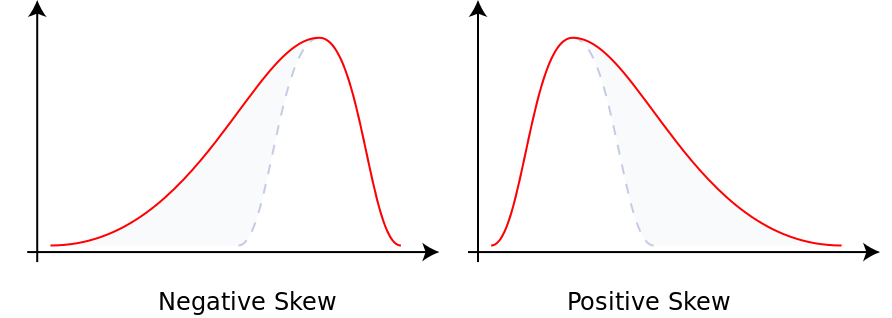
\includegraphics[width=0.6\linewidth,height =0.2\linewidth, angle=0]{skew.png}
        \caption{skewness}
        \label{fig:skewness}
    \end{figure} 
\end{point}

  \begin{point}
    \textbf{kurtosis:} scaled fourth moment \[\mu_4/\sigma^{4}\]
    Kurtosis is a unitless quantity that is often compared to the kurtosis of a normal distribution for context. The term \textbf{excess kurtosis} is often used, meaning kurtosis minus three, since three is the kurtosis of a normal distribution. 
    
    A distribution with positive excess kurtosis is called \textbf{leptokurtic} or \textbf{fat-tailed}, meaning it has more probability attached to unusual observations than a normal distribution. A distribution with zero excess kurtosis is \textbf{mesokurtic}, and a \textbf{thin-tailed} distribution with negative excess kurtosis is called \textbf{platykurtic}.
    
    \textbf{Detail Interpretation:} "...its only unambiguous interpretation is in terms of tail extremity." The logic is simple: Kurtosis is the average (or expected value) of the standardized data raised to the fourth power. Standardized values that are less than 1 (i.e., data within one standard deviation of the mean, where the "peak" would be) contribute virtually nothing to kurtosis, since raising a number that is less than 1 to the fourth power makes it closer to zero. The only data values (observed or observable) that contribute to kurtosis in any meaningful way are those outside the region of the peak; i.e., the outliers that are on tails. Therefore, kurtosis measures outliers/"tail fatness" only; it measures nothing about the "peak". 
\end{point}

\subsection{Exercises}
\begin{problem}\textbf{(Correlation, Gaussian, Multivariate Gaussian)}
    \begin{enumerate}[label=(\alph*)]
        \item If random variables $X$ and $Y$ are Gaussian, then $aX+bY$ is Gaussian only if $X$ and $Y$ are independent or jointly normal (multivariate normally distributed).
        \item If random variables $X$ and $Y$ are Gaussians (not jointly Gaussian), then correlation $0$ does NOT imply independence.
        \item If random variables $X$ and $Y$ are jointly Gaussian, then correlation $0$ DOES imply independence.
        \item Normally distributed and uncorrelated does not imply independent.
    \end{enumerate}    
\end{problem}

\begin{solution}
\begin{enumerate}[label=(\alph*)]
        \item The characteristic function
$$
\varphi_{X+Y}(t)=\mathrm{E}\left(e^{i t(X+Y)}\right)
$$
of the sum of two independent random variables $X$ and $Y$ is just the product of the two separate characteristic functions:
$$
\varphi_X(t)=\mathrm{E}\left(e^{i t X}\right), \quad \varphi_Y(t)=\mathrm{E}\left(e^{i t Y}\right)
$$
of $X$ and $Y$.
The characteristic function of the normal distribution with expected value $\mu$ and variance $\sigma^2$ is
$$
\varphi(t)=\exp \left(i t \mu-\frac{\sigma^2 t^2}{2}\right) \text {. }
$$
So
$$
\begin{aligned}
\varphi_{X+Y}(t)=\varphi_X(t) \varphi_Y(t) & =\exp \left(i t \mu_X-\frac{\sigma_X^2 t^2}{2}\right) \exp \left(i t \mu_Y-\frac{\sigma_Y^2 t^2}{2}\right) \\
& =\exp \left(i t\left(\mu_X+\mu_Y\right)-\frac{\left(\sigma_X^2+\sigma_Y^2\right) t^2}{2}\right) .
\end{aligned}
$$
This is the characteristic function of the normal distribution with expected value $\mu_X+\mu_Y$ and variance $\sigma_X^2+\sigma_Y^2$ Finally, recall that no two distinct distributions can both have the same characteristic function, so the distribution of $X+Y$ must be just this normal distribution.

\item Without loss of generality, we will consider the case of two jointly Gaussian random variables. Extensions to higher dimensions follow by the same reasoning. Suppose that $X_1, X_2$ are uncorrelated. Recall that the entries of the covariance matrix are $\Sigma_{i, j}=\operatorname{cov}\left(X_i, X_j\right)$, which means that
$$
\Sigma=\left[\begin{array}{cc}
\sigma_1^2 & 0 \\
0 & \sigma_2^2
\end{array}\right] \text { and } \Sigma^{-1}=\left[\begin{array}{cc}
1 / \sigma_1^2 & 0 \\
0 & 1 / \sigma_2^2
\end{array}\right]
$$
Substituting $\Sigma^{-1}$ above into the joint PDF, we find that
$$
f_{\mathbf{X}}\left(x_1, x_2\right)=\frac{1}{\sqrt{(2 \pi)^2 \sigma_1^2 \sigma_2^2}} \exp \left(-\frac{1}{2}\left(\frac{\left(x_1-\mu_1\right)^2}{\sigma_1^2}+\frac{\left(x_2-\mu_2\right)^2}{\sigma_2^2}\right)\right)
$$
2
$$
\begin{aligned}
& =\frac{1}{\sqrt{2 \pi \sigma_1^2}} \exp \left(-\frac{1}{2} \frac{\left(x_1-\mu_1\right)^2}{\sigma_1^2}\right) \cdot \frac{1}{\sqrt{2 \pi \sigma_2^2}} \exp \left(-\frac{1}{2} \frac{\left(x_2-\mu_2\right)^2}{\sigma_2^2}\right) \\
& =f_{\mathbf{X}_1}\left(x_1\right) f_{\mathbf{X}_2}\left(x_2\right) .
\end{aligned}
$$

        \item A symmetric example

Suppose $X$ has a normal distribution with expected value 0 and variance 1. Let $W$ have the Rademacher distribution, so that $W=1$ or $W=-1$, each with probability $1 / 2$, and assume $W$ is independent of $X$. Let $Y=W X$. Then
\begin{itemize}
    \item $X$ and $Y$ are uncorrelated;
    \item both have the same normal distribution; and
    \item $X$ and $Y$ are not independent.
\end{itemize}

To see that $X$ and $Y$ are uncorrelated, one may consider the covariance $\operatorname{cov}(X, Y)$ : by definition, it is $\operatorname{cov}(X, Y)=\mathrm{E}(X Y)-\mathrm{E}(X) \mathrm{E}(Y)$.

Then by definition of the random variables $X, Y$, and $W$, and the independence of $W$ from $X$, one has
$$
\operatorname{cov}(X, Y)=\mathrm{E}(X Y)-0=\mathrm{E}\left(X^2 W\right)=\mathrm{E}\left(X^2\right) \mathrm{E}(W)=\mathrm{E}\left(X^2\right) \cdot 0=0 .
$$
To see that $Y$ has the same normal distribution as $X$, consider
$$
\begin{aligned}
\operatorname{Pr}(Y \leq x) & =\mathrm{E}(\operatorname{Pr}(Y \leq x \mid W)) \\
& =\operatorname{Pr}(X \leq x) \operatorname{Pr}(W=1)+\operatorname{Pr}(-X \leq x) \operatorname{Pr}(W=-1) \\
& =\Phi(x) \cdot \frac{1}{2}+\Phi(x) \cdot \frac{1}{2}
\end{aligned}
$$
Joint range of $X$ and $Y$. Darker indicates higher value of the density function.
(since $X$ and $-X$ both have the same normal distribution), where $\Phi(x)$ is the cumulative distribution function of the Standard normal distribution.
To see that $X$ and $Y$ are not independent, observe that $|Y|=|X|$ or that $\operatorname{Pr}(Y>1 \mid-1 / 2<X<1 / 2)=\operatorname{Pr}(X>1 \mid-1 / 2<X<1 / 2)=0$.
Finally, the distribution of the simple linear combination $X+Y$ concentrates positive probability at $0: \operatorname{Pr}(X+Y=0)=1 / 2$. Therefore, the random variable $X+Y$ is not normally distributed, and so also $X$ and $Y$ are not jointly normally distributed (by the definition above).
    \end{enumerate}  
    
\end{solution}




\subsection{Inequalities}
Inequalities are useful in probability for bounding quantities that might otherwise be hard to compute. They are also useful for developing the theory of convergence which is discussed in the next chapter. Our first inequality is Markov's inequality.

\subsubsection{Markov and Chebychev Inequalities}
\begin{theorem}
    \textbf{(Markov's Inequality)}Let $X$ be a non-negative random variable (i.e. $P(X \geq 0)=1)$. Suppose that $E(X)$ exists. For any $t>0$
$$
P(X>t) \leq \frac{E(X)}{t} .
$$
\end{theorem}
\begin{solution}
    We have that \[
    \EE(X)=\int_{0}^{\infty} x f(x) d x=\int_{0}^{t} x f(x) d x+\int_{t}^{\infty} x f(x) d x \geq\int_{t}^{\infty} x f(x) d x \geq t \int_{t}^{\infty} f(x) d x=t P(X>t).\]
\end{solution}

\begin{theorem}
    \textbf{(Chebyshev's inequality)} Let $\mu=E(X)$ and $\sigma^{2}=$ $\operatorname{Var}(X)$. Then,
$$
P(|X-\mu| \geq t) \leq \frac{\sigma^{2}}{t^{2}}
$$
and
$$
P(|Z| \geq k) \leq \frac{1}{k^{2}}
$$
where $Z=(X-\mu) / \sigma$. In particular, $P(|Z|>2) \leq 1 / 4$ and $P(|Z|>3) \leq$ $1 / 9$.
\end{theorem} 

\begin{solution}
    We use Markov's inequality to conclude that
$$
P(|X-\mu| \geq t)=P\left(|X-\mu|^{2} \geq t^{2}\right) \leq \frac{E(X-\mu)^{2}}{t^{2}}=\frac{\sigma^{2}}{t^{2}}
$$
The second part follows by setting $t=k \sigma$.
\end{solution}

\begin{corollary}Let $X_{1}, \ldots, X_{n}$ be $n$ independent random variables with common finite mean $\mu$ and common finite variance $\sigma^{2}$. Let $\bar{X}_{n}=\frac{1}{n} \sum_{i=1}^{n} X_{i}$ and 
$$
Z_{n}=\frac{\left(\bar{X}_{n}-\mu\right)}{\sqrt{\operatorname{Var}\left(\bar{X}_{n}\right)}}=\frac{\sqrt{n}\left(\bar{X}_{n}-\mu\right)}{\sigma}
$$
Then, for $t>0$,
$$
P\left(\left|Z_{n}\right|>t\right) \leq \frac{1}{t^{2}} .
$$
\end{corollary} 

\begin{solution}This follows from the fact that $\operatorname{Var}\left(\bar{X}_{n}\right)=\sigma^{2} / n$ and Chebyshev's inequality.
\end{solution}

\begin{remark}
    Suppose we test a prediction method (a neural net for example) on a set $n=10,000$ new test cases. Let $X_{i}=1$ if the predictor is wrong and $X_{i}=0$ if the predictor is right. Then $\bar{X}_{n}=n^{-1} \sum_{i=1}^{n} X_{i}$ is the observed error rate. Each $X_{i}$ may be regarded as a Bernoulli with unknown mean $p$. We would like to know the true, but unknown error rate $p$. 
    
    Intuitively, we expect that $\bar{X}_{n}$ should be close to $p$. Now, $\mu=\EE X_i=p$ and $\sigma=\sqrt{\operatorname{Var}\left(\mathrm{X}_i\right)}=\sqrt{p(1-p)}$. Let us bound $P(|\bar{X}-p|>.01)$. Using the Chebyshev Inequality, we have
$$
\begin{aligned}
\PP(|\bar{X}-p|>.01) & =\PP\left(\frac{\sqrt{n}\left|\bar{X}_{n}-\mu\right|}{\sigma}>\frac{.01 \sqrt{n}}{\sigma}\right) \\
& =\PP\left(\left|Z_{n}\right|>\frac{1}{\sqrt{p(1-p)}}\right) \\
& \leq p(1-p) \\
& \leq \frac{1}{4} \quad \Longleftarrow \text{since $p(1-p) \leq \frac{1}{4}$ for all $p$}
\end{aligned}
$$
\end{remark} 

\subsubsection{Cauchy-Schwarz and Jensen}

\begin{theorem}
    \textbf{(Cauchy-Schwarz inequality)} If $X$ and $Y$ have finite variances then
$$
\EE|X Y| \leq\sqrt{\EE\left(X^{2}\right) \EE\left(Y^{2}\right)}.
$$
\end{theorem} 

\begin{theorem}
    \textbf{(Jensen's Inequality)} If $g$ is twice differentiable and convex then
$$
\EE g(X) \geq g(\EE X)
$$
If $g$ is concave then
$$
\EE g(X) \leq g(\EE X)
$$
\end{theorem} 
\begin{solution}
    Let $L(x)=a+b x$ be a line, tangent to $g(x)$ at the point $E(X)$. Since $g$ is convex, it lies above the line $L(x)$. So,

$$
\begin{aligned}
\EE g(X) & \geq \EE L(X) =\EE(a+b X) =a+b \EE(X) =L(\EE(X))\xlongequal{\text{tangency}}g(\EE X).
\end{aligned}
$$
\end{solution}

\begin{remark}
    From Jensen's inequality we see that $E X^{2} \geq(E X)^{2}$ and $E(1 / X) \geq$ $1 / E(X)$. Since $\log$ is concave, $E(\log X) \leq \log E(X)$. For example, suppose that $X \sim N(3,1)$. Then $E(1 / X) \geq 1 / 3$.
\end{remark}

\subsubsection{Hoeffding's Inequality}
Recall Markov's inequality. If $X>0$ and $t>0$ then $P(X>t)<E(X) / t$. Hoeffding's Inequality is in the same spirit but it is a sharper inequality. 

\begin{theorem}\textbf{(Hoeffding's Inequality)} Let $Y_{1}, \ldots, Y_{n}$ be independent observations such that $E\left(Y_{i}\right)=0$ and $a_{i} \leq Y_{i} \leq b_{i}$. Let $\epsilon>0$. Then, for any $t>0$,
$$
P\left(\sum_{i=1}^{n} Y_{i} \geq \epsilon\right) \leq e^{-t \epsilon} \prod_{i=1}^{n} e^{t^{2}\left(b_{i}-a_{i}\right)^{2} / 8}
$$
\end{theorem}

\begin{corollary}Let $X_{1}, \ldots, X_{n} \sim \operatorname{Bernoulli}(p)$. Then, for any $\epsilon>0$,
$$
P\left(\left|\bar{X}_{n}-p\right|>\epsilon\right) \leq 2 e^{-2 n \epsilon^{2}}
$$
where $\bar{X}_{n}=n^{-1} \sum_{i=1}^{n} X_{i}$
\end{corollary}
\begin{remark}\hfill

\begin{enumerate}
    \item \textbf{(v.s. Chebyshev)} Recall that $n=10,000$ and $X_{i} \sim \operatorname{Ber}(p)$. Using Chebyshev's inequality we found that
$$
P(|\bar{X}-p|>.01) \leq \frac{1}{4}
$$
According to Hoeffding's inequality,
$$
P(|\bar{X}-p|>.01) \leq 2 e^{-2(.01)^{2} n}=.27
$$
which is roughly the same. In this case, there was not much difference. Often, Hoeffding's inequality gives tighter bounds. 
\item \textbf{(Confidence Interval)} As an aside, let us note that Hoeffding's inequality gives us a simple way to create a confidence interval for a binomial parameter $p$. We will discuss confidence intervals later but let is give the basic idea here. Fix $\alpha>0$ and let
$$
\epsilon_{n}=\left\{\frac{1}{2 n} \log \left(\frac{2}{\alpha}\right)\right\}^{1 / 2}
$$
Hoeffding's inequality says that
$$
P\left(\left|\bar{X}_{n}-p\right|>\epsilon_{n}\right) \leq 2 e^{-2 n \epsilon_{n}^{2}}=\alpha .
$$
Let $C=\left[\bar{X}_{n}-\epsilon, \bar{X}_{n}+\epsilon\right]$. Then, $P(C \notin p)=P\left(\left|\bar{X}_{n}-p\right|>\epsilon\right) \leq \alpha$. Hence, $P(p \in C) \geq 1-\alpha$ that is, the random interval $C$ traps the true parameter value $p$ with probability $1-\alpha$; we call $C$ a $1-\alpha$ confidence interval. 
\end{enumerate}
\end{remark}





  \begin{point}
    \textbf{stochastic dominance:} A random variable $X$ \textbf{first order stochastically dominates} another random variable $Y$ if $F_Y(x)\succeq F_X(x)$ for all scalars $x$.  A standard result is: $X$ stochastically dominates $Y$ if and only if $\mathbb{E}[f(X)]\succeq \mathbb{E}[f(Y)]$ for all increasing functions $f$ where the expectation is defined.

Intuitively, $X$ stochastically dominates $Y$ when $Y$ has more probability associated with low outcomes than $X$ does. Eventually both cumulative distribution functions must get to their highest values ; the value 1. But $Y$ is always in more of a hurry to get to 1 than $X$, meaning $Y$ is always more likely to have a low (disappointing) result than $X$. {\color{C3}$X$ is the better offer.}
    
    \textbf{E.g.} \begin{figure}[!htp]
        \centering
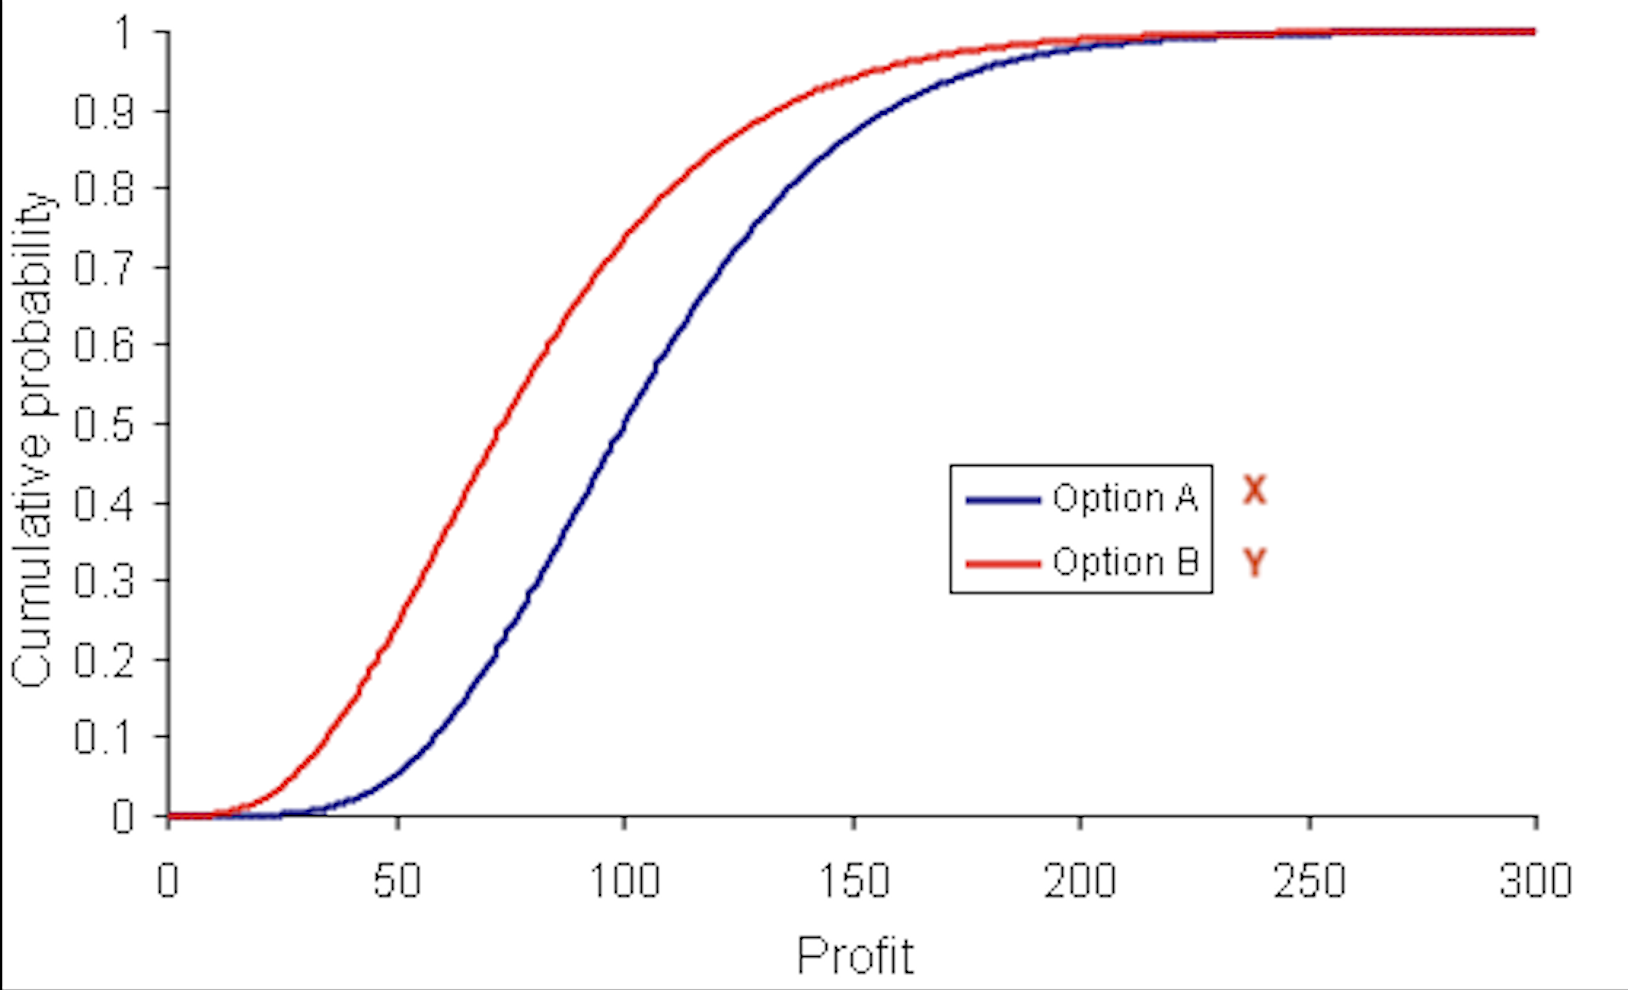
\includegraphics[width=0.4\linewidth,height =0.2\linewidth, angle=0]{stochastic_dominance.png}
        \caption{stochastic dominance}
        \label{fig:stochastic dominance}
    \end{figure} 
\end{point}

\subsection{Covariance}

If X, Y independent, then $Cov(X,Y)=\EE[XY]-\EE[X]\EE[Y]=0$

The reverse is not necessarily true. However if X,Y are jointly Gaussian, then it's true.

\section{Statistics}
\subsection{Parametric Inference}
Suppose we have reason to believe that the distribution from which the data were drawn has a density $f(x ; \theta)$ where $\theta$ is an unknown parameter or a vector of unknown parameters. The problem of inference then reduces to the problem of estimating the parameter $\theta$. In some cases, we might be interested in some function (test statistics) $T(\theta)$. In the next few chapters we discuss how to infer $\theta$ and $T(\theta)$

\subsubsection{Parametric Models}
Suppose we have i.i.d. data $X_{1}, \ldots, X_{n}$ whose pdf (or mass function) is contained in the set
$$
\mathcal{M}=\{f(x ; \theta) ; \theta \in \Theta\}
$$
where $\theta$ is a real number or a vector of real numbers. We call $\theta$ a parameter and $\Theta$ is called the parameter space. The set of $\mathrm{pdf}$ 's, $\mathcal{M}$, is called a parametric statistical model. Our goal is to estimate $\theta$ or some function of $\theta$.

\begin{remark}\hfill 
    \begin{enumerate}
        \item Let $X_{1}, \ldots, X_{n} \sim \operatorname{Bernoulli}(p)$. The parameter is $p$ ($\theta$) and the parameter space is $[0,1]$ ($\Theta$).
        \item Let $X_{1}, \ldots, X_{n} \sim \operatorname{Normal}\left(\mu, \sigma^{2}\right)$. The parameter is $\theta=$ $(\mu, \sigma)$, and the parameter space is $\Theta=\{(\mu, \sigma): \mu \in \mathcal{R}, \sigma>0\}$. Suppose we are interested in estimating the mean of the distribution. We can write the quantity of interest as $T(\mu, \sigma)=\tau$. 
        
        On the other hand, suppose that $X_{i}$ is the outcome of a blood test and suppose we are interested in $\tau$, defined as the fraction of the population whose test score is larger than 1. How do we express this? Let $Z$ denote a standard Normal random variable. Then
$$
\begin{aligned}
\tau =P(X>1) =1-P(X<1) =1-P\left(\frac{X-\mu}{\sigma}<\frac{1-\mu}{\sigma}\right) =1-P\left(Z<\frac{1-\mu}{\sigma}\right) =1-\Phi\left(Z<\frac{1-\mu}{\sigma}\right)
\end{aligned}
$$
Here, we consider $\tau =P(X>1)$ because "fraction of the population whose..."  $\Longleftrightarrow$ "probability of any individual...".

The parameter of interest is $\tau=T(\mu, \sigma)$ where $T(\mu, \sigma)=1-\Phi((1-\mu) / \sigma)$. 

The important point is that the quantity of interest can be thought of as a function of the parameter $\theta$.
\item Recall that $X$ has a $\operatorname{Gamma}(\alpha, \beta)$ distribution if
$$
f(x ; \alpha, \beta)=\frac{1}{\beta^{\alpha} \Gamma(\alpha)} x^{\alpha-1} e^{-x / \beta}, \quad x>0
$$
where $\alpha, \beta>0$ and
$$
\Gamma(\alpha)=\int_{0}^{\infty} y^{\alpha-1} e^{-y} d y
$$
is the Gamma function. {\color{C4}The Gamma distribution is sometimes used to model lifetimes of people, animals, and electronic equipment.} Suppose we want to estimate the average lifetime. The mean of $X_{i}$ is $T(\alpha, \beta)=\alpha / \beta$ since $\EE(X_i)=\alpha / \beta$.
    \end{enumerate}
\end{remark}

\subsubsection{Review of Mean Squared Error and Consistency}
Let $\hat{\theta}_{n}$ be an estimator of $\theta$. Recall that $\hat{\theta}_{n}$ is consistent if $\hat{\theta}_{n} \stackrel{p}{\rightarrow} \theta$. 

Let $\bar{\theta}_{n}=E_{\theta}\left(\widehat{\theta}_{n}\right)$ be the expectation of the estimator $\widehat{\theta}_{n}$. If $\bar{\theta}_{n}=\theta$ we say the estimator is unbiased otherwise it is biased and we define $b_{n} \equiv \bar{\theta}_{n}-\theta$ to be the bias. Bias is not necessarily a bad thing but we would like the bias to get small as the sample size increases. 

Recall that the MSE (mean squared error) is defined by $M S E=E_{\theta}\left(\widehat{\theta}_{n}-\theta\right)^{2}$. Earlier we showed that
$$
M S E=\operatorname{Var}_{\theta}\left(\widehat{\theta_{n}}\right)+\operatorname{bias}^{2} .
$$
If $\operatorname{Var}_{\theta}\left(\widehat{\theta_{n}}\right)$ and bias both tend to 0 , then $\widehat{\theta}_{n} \stackrel{q . m \text {. }}{\rightarrow} \theta$  since $MSE\to 0$ and hence $\widehat{\theta}_{n} \stackrel{p}{\rightarrow} \theta$. 

{\color{C3} So one way to show that $\widehat{\theta}_{n}$ is consistent is to show that the bias and variance go to 0. We will use this way of thinking extensively.}




\subsection{Method of Moments}

\subsection{Maximum Likelihood Estimation}
\begin{problem}\textbf{(Theory of MLE)}
    Suppose $X_1, \ldots, X_n \sim F_\theta\mkern1mu$. 
    Then the likelihood function is 
    \begin{equation*}
        L_n(\theta) = \prod_{i=1}^{n} f_\theta(X_i).
    \end{equation*}

    In your own words, describe the meaning of $L_n(\theta)$ for a specific value of $\theta$ when 
    \begin{enumerate}[label=(\alph*),topsep=0pt]
        \item $f_\theta$ is a probability mass function
        \item $f_\theta$ is a probability density function
    \end{enumerate}
\end{problem}

\begin{solution}
\begin{enumerate}[label=(\alph*),topsep=0pt]
        \item $X\sim F_{\theta}, L(\theta |X_i)=f(X_i|\theta ) = f_{\theta}(X_i) = \PP[X=X_i]$ is the probability of a particular given outcome  $X_i\sim F_{\theta}$ is observed for a $\theta$. $L(\theta |X_i)$ is a function of $\theta$.
        
        Therefore, $L_n(\theta) = \prod_{i=1}^{n} f_\theta(X_i)$ is the total probability of given samples $X_1, X_2, \ldots, X_n\sim F_{\theta}$ are observed for a $\theta$. $L_n(\theta)$ is a function of $\theta$.
        
        In the maximum likelihood estimation, we then want to find $\theta$ such that with this $\theta$, the probability of observing our samples $X_1, X_2, \ldots, X_n$ from $F_{\theta}$ is maximized.
        
        \item $X\sim F_{\theta}, L(\theta |X_i) =f(X_i|\theta )= f_{\theta}(X_i)$ is the probability density of a particular given outcome  $X_i\sim F_{\theta}$ for a $\theta$. $L(\theta |X_i)$ is a function of $\theta$.
        
        Therefore, $L_n(\theta) = \prod_{i=1}^{n} f_\theta(X_i)$ is the joint probability density of given samples $X_1, X_2, \ldots, X_n\sim F_{\theta}$ for a $\theta$. $L_n(\theta)$ is a function of $\theta$.
        
        In the maximum likelihood estimation, we then want to find $\theta$ such that with this $\theta$, the joint probability density of observing our samples $X_1, X_2, \ldots, X_n$ from $F_{\theta}$ is maximized.
        
        \textbf{Why maximizing the joint density?}
        
       Suppose $h>0$, $X\sim F_{\theta}$. $L(\theta |X\in [X_i, X_i+h])=\PP(X\in [X_i, X_i+h]|\theta ) $ is the probability of a particular given outcome  $X\sim F_{\theta}, X\in [X_i, X_i+h]$ is observed for a $\theta$. $L(\theta |X\in [X_i, X_i+h])$ is a function of $\theta$.
       
       Then 
       \begin{align*}
      \arg\max_{\theta} L(\theta |X\in [X_i, X_i+h]) &= \arg\max_{\theta} \frac{1}{h}L(\theta |X\in [X_i, X_i+h]) (h \ \text{is constant}.)\\
      &= \arg\max_{\theta} \frac{1}{h}\PP(X\in [X_i, X_i+h]|\theta )\\
      &= \arg\max_{\theta} \frac{1}{h}\int_{X_i}^{X_i+h} f_{\theta}(x)dx\\     
       \end{align*}
       
       Therefore, we have
       \begin{align*}\arg\max_{\theta}L(\theta |X_i) &=
      \arg\max_{\theta} \left\{\lim_{h\to 0^+}L(\theta |X\in [X_i, X_i+h])\right\}\\ &= \arg\max_{\theta} \left\{\lim_{h\to 0^+}\frac{1}{h}\int_{X_i}^{X_i+h} f_{\theta}(x)dx\right\}\\
      &= \arg\max_{\theta} f_{\theta}(X_i)\\
       \end{align*}
       
       Hence, \textbf{maximizing the probability density $f_{\theta}(X_i)$ amounts to maximizing the likelihood $L(\theta |X_i)$ of the specific observation $X_i$. }
       
       Thus, we'd better just \textbf{define it that way to make it simple and consistent with the discrete case, i.e.}
       \[
       L(\theta |X_i) := f_{\theta}(X_i)
       \]
       and 
       \[
       L_n(\theta)=\prod_{i=1}^{n} L(\theta |X_i) = \prod_{i=1}^{n} f_\theta(X_i).
       \]
       
    \end{enumerate}
\end{solution}

\begin{problem}\textbf{(Bernoulli Distribution)}
    \begin{enumerate}[label=(\alph*),topsep=0pt]
        \item 
            Let $X_1, \ldots, X_n \sim \operatorname{Ber}(p)$ where $p$ is an unknown parameter.
            Show $\ell_n(p) = S\log(p) + (n-S)\log(1-p)$, where $S = X_1 + \cdots + X_n\mkern1mu$, and then find the maximizer of $\ell_n(p)$.
        \item
            Let $X_1, \ldots, X_n \sim N(\mu,\sigma^2)$ where $\mu$ and $\sigma$ are unknown parameters.
            Show $\ell(\mu,\sigma) =c -n\log(\sigma)-nS^2/(2\sigma^2)-n(\bar{X}-\mu)^2/(2\sigma^2)$, where $\bar{X} = n^{-1}(X_1 + \cdots + X_n)$ and then find the maximizer of $\ell_n(\mu,\sigma)$.

    \end{enumerate}
\end{problem}

\begin{solution}
\begin{enumerate}[label=(\alph*),topsep=0pt]
        \item Since $X_i\sim Ber(p)$, we have
        \[
        f_{X_i}(x) = \begin{cases}1 \ \ \  \mathbb{P} = p\\
        0 \ \ \  \mathbb{P}=1-p\end{cases}\Longrightarrow {\color{C3}f_{X_i}(x) = (1-p)^{1-x}p^x}
        \]
        By definition of the likelihood function, we obtain
        \[
        \mathcal{L}_{n}(p) = \prod_{i=1}^n (1-p)^{1-X_i}p^{X_i} = (1-p)^{n-\sum_{i=1}^n X_i}p^{\sum_{i=1}^n X_i}
        \]
        Set $S=\sum_{i=1}^n X_i$, it follows that
        \[
        \Longrightarrow \ell_n(p) = \log(\mathcal{L}_{n}(p)) = \log\left((1-p)^{n-\sum_{i=1}^n X_i}p^{\sum_{i=1}^n X_i}\right) = (n-S)\log(1-p)+ S\log(p)      \]
        
        Therefore, we have
        \[
        \ell_n(p) = (n-S)\log(1-p)+ S\log(p)
        \]
        
        $\ell_n(p)$ is a function of $p$, taking the derivative, we get
        \[
        0=\frac{\partial \ell_n(p)}{\partial p} = -\frac{n-S}{1-p}+\frac{S}{p}\Longrightarrow \hat{p}=p^* = \frac{S}{n}
        \]
        Therefore, the maximizer of $\ell_n(p)$ is $\hat{p}=\frac{S}{n}$.
        \item Since $X_i\sim N(\mu, \sigma^2)$, we have
        \[
        f_{X_i}(x) = \frac{1}{\sqrt{2\pi \sigma^2}}e^{-\frac{1}{2}(\frac{x-\mu}{\sigma})^2}
        \]
        By definition of the likelihood function, we obtain
        \[
        \mathcal{L}_{n}(\mu, \sigma) = \prod_{i=1}^n \frac{1}{\sqrt{2\pi \sigma^2}}e^{-\frac{1}{2}(\frac{X_i-\mu}{\sigma})^2} = \left(\frac{1}{\sqrt{2\pi \sigma^2}}\right)^n e^{-\frac{1}{2}\sum_{i=1}^n(\frac{X_i-\mu}{\sigma})^2}
        \]
        Set $S=\sum_{i=1}^n X_i$, it follows that
        \begin{align*}
        \Longrightarrow \ell_n(\mu, \sigma) = \log(\mathcal{L}_{n}(\mu, \sigma)) &= \log\left(\left(\frac{1}{\sqrt{2\pi \sigma^2}}\right)^n e^{-\frac{1}{2}\sum_{i=1}^n(\frac{X_i-\mu}{\sigma})^2}\right)\\ 
        &= n \log\left(\frac{1}{\sqrt{2\pi \sigma^2}}\right) -\frac{1}{2}\sum_{i=1}^n\left(\frac{X_i-\mu}{\sigma}\right)^2\\
        &=-\frac{n}{2}\log(2\pi) -n\log(\sigma) -\frac{1}{2\sigma^2}\sum_{i=1}^n\left(X_i^2 - 2\mu X_i +\mu^2\right)\\
        &=-\frac{n}{2}\log(2\pi) -n\log(\sigma) -\frac{1}{2\sigma^2}\left(\sum_{i=1}^nX_i^2 - 2\mu \sum_{i=1}^nX_i +n\mu^2\right)\\
        &=-\frac{n}{2}\log(2\pi) -n\log(\sigma) -\frac{n}{2\sigma^2}\left(\mu - \bar{X}_n\right)^2-\frac{n}{2\sigma^2}\left(\frac{\sum_{i=1}^nX_i^2}{n} - \bar{X}_n^2\right)\\
        \text{Set} \ S^2 = \frac{1}{n}\sum_{i=1}^n (X_i-\bar{X}_n)^2\Longrightarrow &= -\frac{n}{2}\log(2\pi) -n\log(\sigma) -\frac{n}{2\sigma^2}\left(\mu - \bar{X}_n\right)^2-\frac{n}{2\sigma^2}S^2\\
        \end{align*}
        
        Therefore, we have
        \[
        \ell_n(\mu, \sigma) = -\frac{n}{2}\log(2\pi) -n\log(\sigma) -\frac{n}{2\sigma^2}\left(\mu - \bar{X}_n\right)^2-\frac{n}{2\sigma^2}S^2
        \]
        where $\bar{X}_n=\frac{1}{n}\sum_{i=1}^n X_i, \ S^2 = \frac{1}{n}\sum_{i=1}^n (X_i-\bar{X}_n)^2$.
        
        $\ell_n(\mu, \sigma)$ is a function of $\mu$ and $\sigma$, taking the partial derivative, we get
        \[
        0=\frac{\partial \ell_n(\mu, \sigma)}{\partial \mu} = -\frac{n}{\sigma^2}(\mu -\bar{X}_n) \Longrightarrow \hat{\mu} = \mu^* = \bar{X}_n
        \]
        \[
        0=\frac{\partial \ell_n(\mu, \sigma)}{\partial \sigma} = -\frac{n}{\sigma} -\frac{nS^2}{2}(-2)\frac{1}{\sigma^3} \Longrightarrow \hat{\sigma} = \sigma^* = S
        \]
        Therefore, the maximizer of $\ell_n(\mu, \sigma)$ is \[\hat{\mu}  = \bar{X}_n =\frac{1}{n}\sum_{i=1}^n X_i \ \ \text{and} \  \ \hat{\sigma} = \sqrt{\frac{1}{n}\sum_{i=1}^n (X_i-\bar{X}_n)^2}.\]
    \end{enumerate}
\end{solution}

\begin{problem}\textbf{(Gamma Distribution)}
    Let $X_1, \ldots, X_n \sim \operatorname{Gamma}(\alpha,\beta)$ where $\alpha$ and $\beta$ are unknown parameters.
    Find the method of moments estimator for $\alpha$ and $\beta$.
\end{problem}

\begin{solution}

Since $X_i\sim Gamma(\alpha, \beta)$, we have
\[
f_{X_i}(x; \alpha, \beta) = \frac{x^{\alpha-1}e^{-\beta x}\beta^\alpha}{\Gamma(\alpha)}, x>0, \alpha, \beta>0
\]
where $\Gamma(\alpha)=(\alpha-1)!$ for integers is the Gamma function.

To find the estimators for $\theta = (\alpha, \beta)$, we have to consider sample moments $\hat{\alpha}_1$ and $\hat{\alpha}_2$.
\[
\hat{\alpha}_1 = \frac{1}{n}\sum_{i=1}^n X_i \ \ \ \text{and} \ \ \ \hat{\alpha}_2 = \frac{1}{n}\sum_{i=1}^n X_i^2
\]
We want to find estimators $\hat{\alpha}, \hat{\beta}$ such that
\[
\left(\alpha_1 = \EE_{\hat{\alpha}, \hat{\beta}}[X]  = \int_0^{\infty} x\cdot \frac{x^{\hat{\alpha}-1}e^{-\hat{\beta}x}\hat{\beta}^{\hat{\alpha}}}{\Gamma(\hat{\alpha})} dx = \frac{\hat{\alpha}}{\hat{\beta}}\right) = \hat{\alpha}_1 = \frac{1}{n}\sum_{i=1}^n X_i
\]
and (by the similar approach)
\[
\left(\alpha_2 = \EE_{\hat{\alpha}, \hat{\beta}}[X^2]  = \int_0^{\infty} x^2\cdot \frac{x^{\hat{\alpha}-1}e^{-\hat{\beta}x}\hat{\beta}^{\hat{\alpha}}}{\Gamma(\hat{\alpha})} dx = \frac{\hat{\alpha}+\hat{\alpha}^2}{\hat{\beta}^2}\right) = \hat{\alpha}_2 = \frac{1}{n}\sum_{i=1}^n X_i^2
\]

\hrule

Here, we use the property $\Gamma(\alpha+1)= \alpha \Gamma(\alpha)$ and have
\[
\int_0^{\infty} x\cdot \frac{x^{\hat{\alpha}-1}e^{-\hat{\beta}x}\hat{\beta}^{\hat{\alpha}}}{\Gamma(\hat{\alpha})} dx= \int_0^{\infty} \frac{\hat{\alpha}}{\hat{\beta}}\cdot \frac{x^{\hat{\alpha}}e^{-\hat{\beta}x}\hat{\beta}^{\hat{\alpha}+1}}{\Gamma(\hat{\alpha}+1)} dx = \frac{\hat{\alpha}}{\hat{\beta}}\int_0^{\infty} f_X(x; \alpha+1, \beta) dx = \frac{\hat{\alpha}}{\hat{\beta}}
\]
and
\[
\int_0^{\infty} x^2\cdot \frac{x^{\hat{\alpha}-1}e^{-\hat{\beta}x}\hat{\beta}^{\hat{\alpha}}}{\Gamma(\hat{\alpha})} dx= \int_0^{\infty} \frac{\hat{\alpha}+\hat{\alpha}^2}{\hat{\beta}^2}\cdot \frac{x^{\hat{\alpha}+1}e^{-\hat{\beta}x}\hat{\beta}^{\hat{\alpha}+2}}{\Gamma(\hat{\alpha}+2)} dx = \frac{\hat{\alpha}+\hat{\alpha}^2}{\hat{\beta}^2}\int_0^{\infty} f_X(x; \alpha+2, \beta) dx = \frac{\hat{\alpha}+\hat{\alpha}^2}{\hat{\beta}^2}
\]
\hrule
Therefore, we get
\begin{align}
    \frac{\hat{\alpha}}{\hat{\beta}}  &= \frac{1}{n}\sum_{i=1}^n X_i\\
    \frac{\hat{\alpha}+\hat{\alpha}^2}{\hat{\beta}^2}  &= \frac{1}{n}\sum_{i=1}^n X_i^2
\end{align}

Set $\bar{X}_n=\frac{1}{n}\sum_{i=1}^n X_i, \ S^2 = \frac{1}{n}\sum_{i=1}^n (X_i-\bar{X}_n)^2$, and by $(1)/[(2)-(1)^2]$, we get
\[
\hat{\beta} = \frac{\frac{1}{n}\sum_{i=1}^n X_i}{\frac{1}{n}\sum_{i=1}^n X_i^2-(\frac{1}{n}\sum_{i=1}^n X_i)^2} = \frac{\bar{X}_n}{\frac{1}{n}\sum_{i=1}^n(X_i-\bar{X}_n)^2} = \frac{\bar{X}_n}{S^2}
\]
Multiply $\hat{\beta}$ by $(1)$ we get
\[
\hat{\alpha}= \frac{\hat{\alpha}}{\hat{\beta}}\cdot \hat{\beta} =\bar{X}_n\cdot \frac{\bar{X}_n}{S^2}  = \frac{\bar{X}_n^2}{S^2}
\]

Hence, the method of moment estimators for $\alpha$ and $\beta$ are
\[
\hat{\alpha}=\frac{\bar{X}_n^2}{S^2}, \ \ \ \hat{\beta} =\frac{\bar{X}_n}{S^2}
\]
where $\bar{X}_n=\frac{1}{n}\sum_{i=1}^n X_i$ and $S^2 = \frac{1}{n}\sum_{i=1}^n (X_i-\bar{X}_n)^2$.
\end{solution}


\begin{problem}\textbf{(Uniform Distribution)}
    Let $X_1, \ldots, X_n \sim \operatorname{Unif}(a,b)$ where $a$ and $b$ are unknown parameters with $a<b$.

    \begin{enumerate}[label=(\alph*),topsep=0pt]
        \item Find the method of moments estimator for $a$ and $b$.
        \item Find the maximum likelihood estimators for $a$ and $b$.
    \end{enumerate}
\end{problem}

\begin{solution}

\begin{enumerate}[label=(\alph*),topsep=0pt]
        \item Since $X_i\sim Unif(a,b)$, we have
        \[
        f_{X_i}(x) = \begin{cases}\frac{1}{b-a} &\forall x\in [a,b]\\
        0  &\forall x\not \in [a,b]\end{cases}
        \]
        
        To find the estimators for $\theta = (a, b)$, we have to consider sample moments $\hat{\alpha}_1$ and $\hat{\alpha}_2$.
\[
\hat{\alpha}_1 = \frac{1}{n}\sum_{i=1}^n X_i \ \ \ \text{and} \ \ \ \hat{\alpha}_2 = \frac{1}{n}\sum_{i=1}^n X_i^2
\]
We want to find estimators $\hat{a}, \hat{b}$ such that
\[
\left(\alpha_1 = \EE_{\hat{a}, \hat{b}}[X]  = \int_{\hat{a}}^{\hat{b}} x\cdot \frac{1}{\hat{b}-\hat{a}} dx = \frac{\hat{a}+\hat{b}}{2}\right) = \hat{\alpha}_1 = \frac{1}{n}\sum_{i=1}^n X_i
\]
and
\[
\left(\alpha_2 = \EE_{\hat{a}, \hat{b}}[X]  = \int_{\hat{a}}^{\hat{b}} x^2\cdot \frac{1}{\hat{b}-\hat{a}} dx = \frac{(\hat{b}-\hat{a})^2}{12}+\frac{(\hat{b}+\hat{a})^2}{4}\right)= \hat{\alpha}_2 = \frac{1}{n}\sum_{i=1}^n X_i^2
\]
Therefore, we get
\begin{align}
    \frac{\hat{a}+\hat{b}}{2}  &= \frac{1}{n}\sum_{i=1}^n X_i\\
    \frac{(\hat{b}-\hat{a})^2}{12}+\frac{(\hat{b}+\hat{a})^2}{4}  &= \frac{1}{n}\sum_{i=1}^n X_i^2
\end{align}

Set $\bar{X}_n=\frac{1}{n}\sum_{i=1}^n X_i, \ S^2 = \frac{1}{n}\sum_{i=1}^n (X_i-\bar{X}_n)^2$, and by $\sqrt{3[(4)-(3)^2]}+(3)$, we get
\[
\hat{b} = \frac{1}{n}\sum_{i=1}^n X_i+\sqrt{3}\sqrt{\frac{1}{n}\sum_{i=1}^n X_i^2-(\frac{1}{n}\sum_{i=1}^n X_i)^2}= \bar{X}_n+ \sqrt{3}S
\]
Solve $\hat{a}$ by $(3)$ we get
\[
\hat{a}= 2\cdot \frac{\hat{a}+\hat{b}}{2} -\hat{b}  =2\cdot \bar{X}_n-\bar{X}_n- \sqrt{3}S= \bar{X}_n- \sqrt{3}S
\]

Hence, the method of moment estimators for $a$ and $b$ are
\[
\hat{a}= \bar{X}_n- \sqrt{3}S, \ \ \ \hat{b}  =\bar{X}_n+ \sqrt{3}S
\]
where $\bar{X}_n=\frac{1}{n}\sum_{i=1}^n X_i$ and $S^2 = \frac{1}{n}\sum_{i=1}^n (X_i-\bar{X}_n)^2$.
        \item WLOG, assume we have $X_1\le X_2\le \cdots X_n$. 
        
        Since $X_i\sim Unif(a,b)$, we have
        \[
        f_{X_i}(x) = \begin{cases}\frac{1}{b-a} &\forall x\in [a,b]\\
        0  &\forall x\not \in [a,b]\end{cases}
        \]
        
        By the definition of the likelihood function, we obtain
        \[\mathcal{L}_n(a,b) =\begin{cases}\prod_{i=1}^n \frac{1}{b-a} &\forall i, X_i\in [a,b]\\
        0  &\text{otherwise}\end{cases} = \begin{cases} \frac{1}{(b-a)^n} &\forall i, X_i\in [a,b]\\
        0  &\text{otherwise}\end{cases}
        \]
        
        It follows that
        \[
        \frac{\partial \mathcal{L}_n(a,b) }{\partial a} =\begin{cases} \frac{n}{(b-a)^{n+1}}>0 &\forall a \le \min\{X_1, X_2, \ldots ,X_n\}\\
        0 &\text{otherwise}\end{cases}\Longrightarrow \hat{a} = a^* = \min\{X_1, X_2, \ldots ,X_n\}
        \]
        and
        \[
        \frac{\partial \mathcal{L}_n(a,b) }{\partial b} =\begin{cases} -\frac{n}{(b-a)^{n+1}}<0 &\forall b \ge \max\{X_1, X_2, \ldots ,X_n\}\\
        0 &\text{otherwise}\end{cases}\Longrightarrow \hat{b} = b^* = \max\{X_1, X_2, \ldots ,X_n\}
        \]
        Therefore, the maximum likelihood estimators of $a,b$ are
        \[
        \hat{a}  = \min\{X_1, X_2, \ldots ,X_n\}, \quad \hat{b} = \max\{X_1, X_2, \ldots ,X_n\}
        \]
    \end{enumerate}

\end{solution}    

\newpage    
\begin{problem}\textbf{(Poisson Distribution)}
    Let $X_1, \ldots, X_n \sim \operatorname{Poisson}(\lambda)$ where $\lambda$ is an unknown parameter.

    \begin{enumerate}[label=(\alph*),topsep=0pt]
        \item Find the method of moments estimator for $\lambda$.
        \item Find the maximum likelihood estimators for $\lambda$.
    \end{enumerate}
\end{problem}

\begin{solution}
\begin{enumerate}[label=(\alph*),topsep=0pt]
        \item Since $X_i\sim Poisson(\lambda)$, we have
        \[
        f_{X_i}(k;\lambda) =\PP[X_i=k] = e^{-\lambda}\frac{\lambda^k}{k!}, \quad k\in \mathbb{N}
        \]
        
        To find the estimators for $\theta = (\lambda)$, we have to consider sample moment $\hat{\alpha}_1$.
\[
\hat{\alpha}_1 = \frac{1}{n}\sum_{i=1}^n X_i 
\]
We want to find estimators $\hat{\lambda}$ such that
\[
\left(\alpha_1 = \EE_{\hat{\lambda}}[X]  = \sum_{k=0}^{\infty} k\cdot e^{-\hat{\lambda}}\frac{\hat{\lambda}^k}{k!} =\hat{\lambda}e^{-\hat{\lambda}}\sum_{l=0}^{\infty}  \frac{\hat{\lambda}^{l}}{l!}=\hat{\lambda}e^{-\hat{\lambda}}e^{\hat{\lambda}}= \hat{\lambda}\right) = \hat{\alpha}_1 = \frac{1}{n}\sum_{i=1}^n X_i
\]

Therefore, we get
\begin{align}
    \hat{\lambda}  &= \frac{1}{n}\sum_{i=1}^n X_i
\end{align}

Set $\bar{X}_n=\frac{1}{n}\sum_{i=1}^n X_i$, and we can conclude that the method of moment estimator for $\lambda$ is
\[
\hat{\lambda} = \bar{X}_n
\]
where $\bar{X}_n=\frac{1}{n}\sum_{i=1}^n X_i$.
        \item WLOG, assume we have $X_1\le X_2\le \cdots X_n$. 
        
        Since $X_i\sim Poisson(\lambda)$, we have
        \[
        f_{X_i}(k;\lambda) =\PP[X_i=k] = e^{-\lambda}\frac{\lambda^k}{k!}, \quad k\in \mathbb{N}
        \]
        
        By the definition of the likelihood function, we obtain
        \[\mathcal{L}_n(\lambda) =\prod_{i=1}^n e^{-\lambda}\frac{\lambda^{X_i}}{X_i!} = \frac{e^{-n\lambda}\lambda^{\sum_{i=1}^n X_i}}{\prod_{i=1}^n X_i!}
        \]
        \[
        \Longrightarrow \ell_n(\lambda) = \log(\mathcal{L}_n(\lambda)) = -n\lambda + (\sum_{i=1}^n X_i)\log(\lambda) - \log(\prod_{i=1}^n X_i!)
        \]
        
        It follows that
        \[
        0=\frac{\partial \ell_n(\lambda) }{\partial \lambda} =-n +\frac{1}{\lambda}(\sum_{i=1}^n X_i) \Longrightarrow \hat{\lambda} = \lambda^* = \frac{1}{n}\sum_{i=1}^n X_i = \bar{X}_n
        \]
        where $\bar{X}_n=\frac{1}{n}\sum_{i=1}^n X_i$.
        
        Therefore, the maximum likelihood estimator of $\lambda$ is
        \[
        \hat{\lambda}  = \bar{X}_n
        \]
    \end{enumerate}

\end{solution}

\newpage
\begin{problem}\textbf{(Invariance of MLE)}
    Let $X_1, \ldots, X_n \sim N(\theta,1)$ where $\theta$ is an unknown parameter.
    Define
    \begin{equation*}
        Y_i = \begin{cases}1 & X_i > 0 \\ 0 & X_i \leq 0. \end{cases}
    \end{equation*}
    Let $\psi = \PP[Y_1 = 1]$.

    Find the maximum likelihood estimator for $\psi$.
\end{problem}

\begin{solution}
By the definition, we have
\begin{align*}
\psi = \PP[Y_1= 1] = \PP[X_1>0] =\PP[X_1-\theta>-\theta]= 1-\Phi(-\theta) = \Phi(\theta)  = g(\theta)
\end{align*}
where $\Phi$ is the CDF of $Z\sim N(0,1)$.

Then, by the equivariance property of the maximum likelihood estimator, we know that if $\hat{\theta}$ is a MLE of $\theta$, then $g(\hat{\theta})$ is a MLE of $g(\theta)$. Now, let's find the MLE $\hat{\theta}$
of $\theta$.

By the definition of the likelihood function, we get
\[
\mathcal{L}_n(\theta) = \prod_{i=1}^n  \frac{1}{\sqrt{2\pi}}e^{-\frac{1}{2}\left(X_i-\theta\right)^2} = \left(\frac{1}{\sqrt{2\pi}}\right)^n e^{-\frac{1}{2}\sum_{i=1}^n (X_i-\theta)^2}
\]
\[
\Longrightarrow \ell_n(\theta) = n\log\left(\frac{1}{\sqrt{2\pi}}\right)-\frac{1}{2}\sum_{i=1}^n (X_i-\theta)^2
\]
\[
\Longrightarrow 0=\frac{\partial \ell_n(\theta)}{\theta} = \sum_{i=1}^n (X_i-\theta) = -n\theta+\sum_{i=1}^n X_i \Longrightarrow \hat{\theta}=\theta^* = \frac{1}{n}\sum_{i=1}^n X_i = \bar{X}_n
\]
where $\bar{X}_n = \frac{1}{n}\sum_{i=1}^n X_i$.

Therefore, the MLE $\hat{\psi}$ for $\psi$ is 
\[
\hat{\psi} = g(\hat{\theta}) = \Phi(\hat{\theta}) = \Phi(\bar{X}_n)
\]
\end{solution}

\subsection{Statistical Tests}
\subsubsection{Chi-square Test}


\subsubsection{Split Histogram -- Test for Identical Distribution}


\subsubsection{Lag Plot -- Test for Independence}


\subsection{Hypothesis Testing}
\textbf{Hypothesis}
\begin{enumerate}[label=\textbullet]
    \item $H_0 = \{\theta \in \Theta\}$: Null Hypothesis. E.g. "Given email is not a spam."
    \item $H_1= \{\theta \in \Theta^{C}\}$: Alternative Hypothesis. E.g."Given email is spam."
\end{enumerate}
{\color{C3} $H_0$ will normally be be hypothesis you deem as true and want to test.}

\textbf{Hypothesis Test Tools}
\begin{enumerate}[label=(\arabic*)]
    \item Given data $X_1, X_2, \ldots, X_n \sim F_{\theta}$ sampled from distribution $F_{\theta}$.
    \item Construct \textbf{test statistics} $T(X_1, X_2, \ldots, X_n)$.
    \item Construct \textbf{rejection region} $R=\{(X_1, X_2, \ldots, X_n)|T(X_1, X_2, \ldots, X_n)>c\}$ where $c$ is a constant threshold.

    \[\begin{cases}
    \text{If}  ~(X_1, X_2, \ldots, X_n)\in R, \text{reject} H_0,\\
    \text{If}  ~(X_1, X_2, \ldots, X_n)\not\in R, \text{fail to reject} H_0.
    \end{cases}\]
    \item Define \textbf{power function} of a test with associated rejection region to be $\beta(\theta) = \PP[T(X_1, X_2, \ldots, X_n)>c|X_1, X_2, \ldots, X_n\sim F_{\theta}]$. 

    \textbf{Interpretation:} Assuming $H_0=\{\theta\in\Theta\}$ is true, and we have constructed the test statistics $T$ and rejection region $R$, the probability of $(X_1, X_2, \ldots, X_n)$ being in the rejection region $R$ is $\beta(\theta)$. (or the probability of rejecting $H_0$ is a mistake is $\beta(\theta)$.
    \item Define the \textbf{size} of the test $\alpha = \sup_{\theta\in\Theta} \beta(\theta)$. That is 
    \[
    \alpha = \sup_{\theta\in\Theta}\PP[T(X_1, X_2, \ldots, X_n)>c_{\alpha}|X_1, X_2, \ldots, X_n]
    \]

    \textbf{Interpretation:}
    \begin{enumerate}[label=(\alph*)]
    \item For our sampled data $X_1, X_2, \ldots, X_n$  given $H_0$ is true, we should NOT reject it, but there is still a possibility that the test statistics would be in $R$. 
    
    We then want to know given our sampled data $X_1, X_2, \ldots, X_n$  and $H_0$ being true, if we set a rejection region $R$, what is the maximum probability that the test statistics will be in the rejection region $R$ (i.e. the maximum probability that we will make the mistake of rejecting $H_0$ given $H_0$ being true.) 

    That's why we want to analyze $\alpha$.
        \item Assuming $H_0$ is true, {\color{C2}for a rejection region \[R=\{(X_1, X_2, \ldots, X_n):T(X_1, X_2, \ldots, X_n)>c_{\alpha}\},\] the corresponding $\alpha$ is the maximum probability that rejecting $H_0$ is a mistake (or the maximum probability of making the type I error)}.
        \item $\alpha$ and $c$ has a one-to-one mapping relationship; that is $\alpha = g(c)$, so we usually write $c$ as $c_{\alpha}$ to underscore that.
        \item Normally $\alpha \propto \frac{1}{c_{\alpha}}$. We can see below, as the threshold $c_{\alpha}$ increases (move to the right), the corresponding $\alpha$ (the shaded region) becomes smaller, and vice versa.
    \end{enumerate}
\end{enumerate}

\begin{center}
    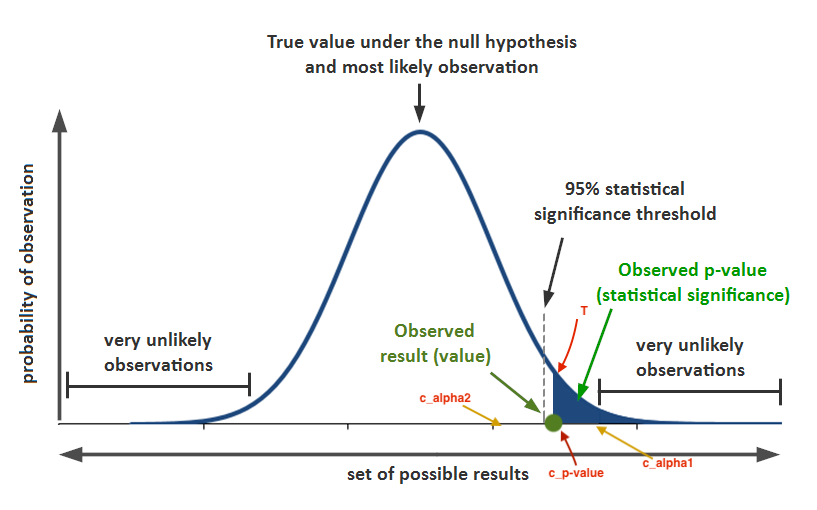
\includegraphics[width=0.8\textwidth]{p_value.png}
    \end{center}
\textbf{Hypothesis Test Idea:}

Assume the null hypothesis $H_0$ is true. 

If there exists a rejection region $R$ which can reject the data $X_1, X_2, \ldots, X_n$ sampled from $F_{\theta}$ (i.e. $(X_1, X_2, \ldots, X_n)\in R$), and the corresponding $\alpha$ -- the maximum probability that rejecting $H_0$ is a mistake is $<0.05$, then we say we are confident enough to reject $H_0$; that is $H_0$ is very very likely to be false. Otherwise, we say that we don't have enough evidence to reject $H_0$.

\begin{remark}\hfill
\begin{enumerate}
    \item Normally, the smallest threshold $c_{\alpha}=T(X_1, X_2, \ldots, X_n)$, and the corresponding $\alpha$ is the $p-value$. That is $c_{p-value}=T(X_1, \ldots, X_n)$. (See figure above.)
    \item When we say that we don't have enough evidence to reject $H_0$, it does NOT necessarily suggests that $H_0$ is true.
\end{enumerate}
\end{remark}

With this idea, we define the \textbf{p-value} as
\[
p-value = \inf\{\alpha: T(X_1, X_2, \ldots, X_n)>c_{\alpha}|X_1, X_2, \ldots, X_n\}
\]
{\color{C3} So, the $p-value$ is a probability.}

\textbf{Interpretation:}

Assuming $H_0$ is true. Given samples $X_1, X_2, \ldots, X_n$, the $p-value$ is the smallest among all $\alpha$'s -- the maximum probability that rejecting $H_0$ is a mistake. (So if $p-value$ is $<0.05$, then there at least exists $1$ rejection region that given this rejection region we can say have only $<0.05$ probability that rejecting $H_0$ is a mistake.)

The smaller the $p-value$, the smaller the maximum probability that rejecting $H_0$ is a mistake is. Then the more confident we are in rejecting $H_0$.

$p-value$是获得样本$X_1, X_2, \ldots, X_n$的情况下,拒绝$H_0$是犯第一类错误的最大概率中最小的那个。

$p-value$越小,我们拒绝$H_0$是犯第一类错误的最大概率越小。那么我们就越有信心拒绝$H_0$。

So, if $p-value<0.05$, it suggests that there exists a rejection region $R$ that can reject $H_0$ for the given samples $X_1, X_2, \ldots, X_n$, and the maximum probability of making the rejection decision is a mistake is only $5\%$. So we should be confident enough to reject $H_0$.
\begin{remark}
    Informally, we can just say:

    Assuming $H_0$ is true. Given samples $X_1, X_2, \ldots, X_n$, the $p-value$ is the maximum probability that rejecting $H_0$ is a mistake.
\end{remark}
\textbf{Hypothesis Test Procedure}

\begin{enumerate}
    \item Set Null Hypothesis $H_0$ and Alternative Hypothesis $H_1$.
    \item Get samples $X_1, X_2, \ldots, X_n$.
    \item Set test statistics $T$ and rejection region $R$.
    \item Find the relationship between the rejection threshold $c_{\alpha}$ and $\alpha$. Normally $\alpha = g(c_{\alpha})$, and $g$ is monotone decreasing.
    \item Plug $c_{p-value} = T(X_1, X_2, \ldots, X_n)$ in to $\alpha = g(c_{\alpha})$, and we get
    \[
    p-value=g(c_{p-value})=g(T(X_1, X_2, \ldots, X_n))
    \]
    \item Then check if $p-value$ is $<0.05$.
\end{enumerate}

\begin{theorem}
    p-value is uniformly distributed.
\end{theorem}

\begin{solution}
    Assume $H_0$ is true, you have your test statistics and $T(X_1, X_2, \ldots, X_n)$ and suppose the CDF of the test statistics is $F$. By definition, we have
    \[
    \alpha = \sup_{\theta\in\Theta}\PP[T(X_1, X_2, \ldots, X_n)>c_{\alpha}|X_1, X_2, \ldots, X_n] = 1- F_{\theta^*}(c_{\alpha})
    \]
    Since $c_{p-value} = T(X_1, X_2, \ldots, X_n)$, we have
    \[
    p-value = 1- F_{\theta^*}(T(X_1, X_2, \ldots, X_n))
    \]
    Then 
    \begin{align*}
        \PP[p-value<p] &= \PP[1- F_{\theta^*}(T(X_1, X_2, \ldots, X_n))<p]\\
        &= \PP[1-p< F_{\theta^*}(T(X_1, X_2, \ldots, X_n))]\\
        &=\PP[F_{\theta^*}^{-1}(1-p)< T(X_1, X_2, \ldots, X_n)]\\
        \text{$F$ is the CDF of $T$}\Longrightarrow&=1-F(F_{\theta^*}^{-1}(1-p))\\
        &=p
    \end{align*}
    Therefore, we have $\PP[p-value<p]=p$. That just suggests the p-value is uniformly distributed.
\end{solution}



\subsection{Exercises}
\begin{problem}
Suppose that the size $\alpha$ test is of the form
    \begin{equation*}
        \text{reject $H_0=\{\theta\in\Theta_0\}$ if and only if $T(X_1, \ldots, X_n) > c_\alpha$}.
    \end{equation*}

    \begin{enumerate}[label=(\alph*),topsep=0pt]
        \item Given data $X_1, \ldots, X_n\mkern1mu$, prove that, 
    \begin{equation*}
        \text{$p$-value} = \sup_{\theta\in\Theta_0} \PP[T(X_1', \ldots, X_n') > T(X_1, \ldots, X_n) | X_1', \ldots, X_n' \sim F_\theta].
    \end{equation*}
    \item Explain, in simple words, what this result says about the meaning of a $p$-value for this type of test.
    \end{enumerate}
\end{problem}

\begin{solution}
\begin{enumerate}[label=(\alph*),topsep=0pt]
    \item By definition, we have
    \begin{align*}
    p-value &= inf_{\alpha}\{\alpha: T(X_1, \ldots, X_n) >c_{\alpha}|X_1, \ldots, X_n \sim F_\theta\}\\
    &= sup_{\theta\in \Theta_0}\PP[ T(X_1', \ldots, X_n') >c_{p-value}|X_1', \ldots, X_n' \sim F_\theta]\\
   c_{p-value}=T(X_1, \ldots, X_n) \Longrightarrow &= sup_{\theta\in \Theta_0}\PP[ T(X_1', \ldots, X_n') >T(X_1, \ldots, X_n)|X_1', \ldots, X_n' \sim F_\theta]\\
\end{align*}
\[\Longrightarrow p-value =sup_{\theta\in \Theta_0}\PP[ T(X_1', \ldots, X_n') >T(X_1, \ldots, X_n)|X_1', \ldots, X_n' \sim F_\theta]\]
    \item Suppose hypothesis $H_0$ is true, the p-value is the probability of observing a value of the test statistic more extreme than what was actually observed.
    \end{enumerate}
\end{solution}

\begin{problem}[Wasserman 10.5]
    Let $X_1, \ldots, X_n\sim \operatorname{Unif}(0,\theta)$ and let $Y=\max\{X_1, \ldots, X_n\}$.
    We want to test $H_0 = \{ \theta  \leq 1/2 \}$ vs $H_1 = \{\theta>1/2\}$ and we will reject if $Y>c$ for some constant $c$.
    \begin{enumerate}[label=(\alph*),topsep=0pt]
        \item Find the power function $\beta(\theta) = \PP[\max\{X_1, \ldots, X_n\} > c | X_1, \ldots, X_n \sim \operatorname{Unif}(0,\theta) ]$.
        \item What choice of $c$ will make the size of the test $0.05$?
        \item In a sample of size $n=20$ with $Y=0.48$, what is the $p$-value? What is the conclusion about $H_0$ that you would make?
        \item In a sample of size $n=5$ with $Y=0.45$, what is the $p$-value? What is the conclusion about $H_0$ that you would make? Since $Y=0.45$ is smaller than the previous case, we might expect it would be ``harder to reject'' $H_0$, yet the $p$-value is smaller than the previous case. 
            Explain this observation. 
        \item In a sample of size $n=20$ with $Y=0.52$, what is the $p$-value? What is the conclusion about $H_0$ that you would make?
    \end{enumerate}

\end{problem}

\begin{solution}
\begin{enumerate}[label=(\alph*),topsep=0pt]
    \item We have \begin{align*}\beta(\theta) &= \PP[\max\{X_1, \ldots, X_n\} > c | X_1, \ldots, X_n \sim \operatorname{Unif}(0,\theta)]\\
    &= 1-\PP[\max\{X_1, \ldots, X_n\} \le c | X_1, \ldots, X_n \sim \operatorname{Unif}(0,\theta)]\\
    &= 1-\PP[(X_1\le c)\cap \cdots \cap\PP(X_n\le c) | X_1, \ldots, X_n \sim \operatorname{Unif}(0,\theta)]\\
    &= 1-\prod_{i=1}^n\PP[X_i\le c| X_i\sim \operatorname{Unif}(0,\theta)]\\
    &= \begin{cases}
    0 \quad & \text{if}\quad c>\theta\\
    1-\left(\frac{c}{\theta}\right)^n \quad & \text{if}\quad c \in [0, \theta]\\
    1 \quad & \text{if}\quad c<0\\
    \end{cases}
    \end{align*}
    
    Therefore, the power function is
    \[
    \beta(\theta)= \begin{cases}
    0 \quad & \text{if}\quad c>\theta\\
    1-\left(\frac{c}{\theta}\right)^n \quad & \text{if}\quad c \in [0, \theta]\\
    1 \quad & \text{if}\quad c<0\\
    \end{cases}
    \]
    \item By definition, the size of the test is 
    \[size = \sup_{\theta\in\Theta_0}\beta(\theta)\]
    where $\Theta_0 = \{\theta: 0\le \theta\le \frac{1}{2}\}$.
    
    Then we have
    \[
    \alpha =0.05 = size = \sup_{\theta\in\Theta_0}\beta(\theta) = \begin{cases}
    0 \quad & \text{if}\quad c>\theta\\
    1-\left(2c\right)^n \quad & \text{if}\quad c \in [0, \theta]\\
    1 \quad & \text{if}\quad c<0\\
    \end{cases} \Longrightarrow c = \frac{1}{2}\sqrt[n]{0.95}
    \]
    
    Therefore, we should pick $c=\frac{1}{2}\sqrt[n]{0.95}$.
    \item By the definition, we have
    \begin{align*}
        p-value &= \inf_{\alpha}\{\alpha: \max\{X_1, \ldots, X_n\} > c_{\alpha} | X_1, \ldots, X_n \sim \operatorname{Unif}(0,\theta)\}\\
        &= \inf_{\alpha}\{\alpha: 0.48> \frac{1}{2}\sqrt[n]{1-\alpha}\}\\
        &= \inf_{\alpha}\{\alpha: \alpha> 1- (2*0.48)^n \}\\
        n=20 \Longrightarrow &= \inf_{\alpha}\{\alpha: \alpha> 1- (2*0.48)^{20} \}\\
        &=0.558
    \end{align*}
    
    Therefore, the p-value is $0.558$, and since it's pretty large, we cannot really reject $H_0$.
    \item By the same logic as (c), we get
    
    \begin{align*}
        p-value &= \inf_{\alpha}\{\alpha: \max\{X_1, \ldots, X_n\} > c_{\alpha} | X_1, \ldots, X_n \sim \operatorname{Unif}(0,\theta)\}\\
        &= \inf_{\alpha}\{\alpha: 0.45> \frac{1}{2}\sqrt[n]{1-\alpha}\}\\
        &= \inf_{\alpha}\{\alpha: \alpha> 1- (2*0.45)^n \}\\
        n=5 \Longrightarrow &= \inf_{\alpha}\{\alpha: \alpha> 1-(2*0.45)^{5} \}\\
        &=0.410
    \end{align*}
    
    Therefore, the p-value is $0.410$, and since it's pretty large, we cannot really reject $H_0$.
    
    I think the reason that the p-value is smaller than the previous one is because the sample size $n$ is smaller.
    \item By the same logic, we have
    \begin{align*}
        p-value &= \inf_{\alpha}\{\alpha: \max\{X_1, \ldots, X_n\} > c_{\alpha} | X_1, \ldots, X_n \sim \operatorname{Unif}(0,\theta)\}\\
        &= \inf_{\alpha}\{\alpha: 0.52> \frac{1}{2}\sqrt[n]{1-\alpha}\}\\
        &= \inf_{\alpha}\{\alpha: \alpha> 1- (2*0.52)^n \}\\
        n=20 \Longrightarrow &= \inf_{\alpha}\{\alpha: \alpha> 1-(2*0.52)^{20} \}\\
        &=0
    \end{align*}
    
    In this case, we reject $H_0$. 
    \end{enumerate}
\end{solution}


\begin{problem}[Wasserman 10.6]
There is a theory that people can postpone their death until after an  important event. To test the theory, Phillips and King (1988) collected  data on deaths around the Jewish holiday Passover. 
Of 1919 deaths, 922  died the week before the holiday and 997 died the week after. 

    We can model this situation by thinking of whether each person died after or before the holiday as an iid Bernoulli random variable with parameter $p$.
    Then, the number of people who died after the holiday is a Binomial random variable with parameter $(n,p)$, where $n=1919$.

    \begin{enumerate}[label=(\alph*),topsep=0pt]
        \item for each $\alpha\in(0,1)$, devise a size-$\alpha$ test for the null hypothesis that $p = 1/2$. 
        \item Report and  interpret the $p$-value. 
        \item Construct a confidence interval for $p$.
    \end{enumerate}
\end{problem}

\begin{solution}

Suppose $X_i \sim Ber(p) = \begin{cases}0 \quad \PP = 1-p\\
1 \quad \PP = p\end{cases}, i=1,2,\ldots, 1919$.

where $0 \longrightarrow \text{died before holiday}; 1\longrightarrow \text{didn't die before holiday}$.

\[H_0: p=\frac{1}{2}; \quad H_1: p\not =\frac{1}{2}\]

Set $\bar{X}_n = \frac{1}{n}\sum_{i=1}^n X_i$, then $\bar{X}_n\sim N\left(p, \frac{\PP(1-p)}{n}\right)$.


\begin{enumerate}[label=(\alph*),topsep=0pt]
    \item Construct test statistics to be 
    \[
    T(X_1, \ldots, X_n) = \left|\frac{\bar{X}_n -p}{\sqrt{\VV[\bar{X}_n]}}\right|
    \]
    Then the rejection region is 
    \[
    R = \left\{\left|\frac{\bar{X}_n -p}{\sqrt{\VV[\bar{X}_n]}}\right|>c \Big|X_1, \ldots, X_n\sim Ber(p)\right\}
    \]
    By definition, we have
    \begin{align*}
        \alpha = size &= \sup_{p=\frac{1}{2}}\beta(p)\\
        &= \sup_{p=\frac{1}{2}}\PP[T(X_1, \ldots, X_n) > c]\\
        &= \sup_{p=\frac{1}{2}}\PP\left[\left|\frac{\bar{X}_n -p}{\sqrt{\VV[\bar{X}_n]}}\right| > c\right]\\
        &= \sup_{p=\frac{1}{2}}\PP\left[\frac{\bar{X}_n -p}{\sqrt{\VV[\bar{X}_n]}} > c\right]+\PP\left[\frac{\bar{X}_n -p}{\sqrt{\VV[\bar{X}_n]}} < -c\right]\\
        &= \sup_{p=\frac{1}{2}}2\Phi(-c)\\
        &= 2\Phi(-c)\\
    \end{align*}
    Then, for a given $\alpha\in (0,1)$, the size-$\alpha$ test will be 
    \[
    R = \left\{T(X_1,\ldots, X_n)>-\Phi^{-1}\left(\frac{1}{2}\alpha\right) \Big|X_1, \ldots, X_n\sim Ber(p)\right\}
    \]
    where $T(X_1, \ldots, X_n) = \left|\frac{\bar{X}_n -p}{\sqrt{\VV[\bar{X}_n]}}\right|$.
    \item From the question, we know that $\bar{X}_n = \frac{997}{1919}$, then \[T(X_1, \ldots, X_n) = \left|\frac{\bar{X}_n -p}{\sqrt{\VV[\bar{X}_n]}}\right|=\sqrt{1919}\left|\frac{\frac{997}{1919} -\frac{1}{2}}{\sqrt{\frac{1}{2}(1-\frac{1}{2})}}\right| = \frac{75}{\sqrt{1919}}.\]
    
    Then, by definition, we get
    \begin{align*}
        p-value &= \inf_{\alpha}\{\alpha:T(X_1, \ldots, X_n)>c_{\alpha}\Big|X_1, \ldots, X_n\sim Ber(p)\}\\
        &= \inf_{\alpha}\{\alpha:T(X_1, \ldots, X_n)>-\Phi^{-1}\left(\frac{1}{2}\alpha\right)\Big|X_1, \ldots, X_n\sim Ber(p)\}\\
        &= \inf_{\alpha}\{\alpha:\frac{75}{\sqrt{1919}}>-\Phi^{-1}\left(\frac{1}{2}\alpha\right)\Big|X_1, \ldots, X_n\sim Ber(p)\}\\
         &= \inf_{\alpha}\{\alpha:\alpha > 2\cdot \Phi\left(-\frac{75}{\sqrt{1919}}\right)\Big|X_1, \ldots, X_n\sim Ber(p)\}\\
         &= \inf_{\alpha}\{\alpha:\alpha > 0.0869\Big|X_1, \ldots, X_n\sim Ber(p)\}\\
    \end{align*}
    
    Therefore, the p-value is $0.0869$, and this provides a weak evidence against $H_0$.
    \item Since $\bar{X}_n\sim N\left(p, \frac{\PP(1-p)}{n}\right)$, we have $\frac{\bar{X}_n -p}{\sqrt{\VV[\bar{X}_n]}}\sim N(0,1)$.
    Then
    \[
    \PP\left(\left|\frac{\bar{X}_n -p}{\hat{se}}\right|<c\right)\approx\PP\left(\left|\frac{\bar{X}_n -p}{\sqrt{\VV[\bar{X}_n]}}\right|<c\right)=\PP\left(\left|Z\right|<c\right)=\Phi(c)-\Phi(-c)=2\Phi(c)-1=1-\alpha
    \]
    where $Z\sim N(0,1)$.
    
    We pick $c=\Phi^{-1}\left(1-\frac{1}{2}\alpha\right)$, we get a $1-\alpha$ confidence interval
    \[
    \left(-\hat{se}\Phi^{-1}\left(1-\frac{1}{2}\alpha\right)+\bar{X}_n, \hat{se}\Phi^{-1}\left(1-\frac{1}{2}\alpha\right)+\bar{X}_n\right)
    \]
    where $\bar{X}_n=\frac{997}{1919}$ and $\hat{se}=\sqrt{\frac{(\bar{X}_n)(1-\bar{X}_n)}{1919}}=0.0114$.
    \end{enumerate}
\end{solution}

\begin{problem}
Suppose you work for a pharmaceutical company.
You are trying to develop drugs to reduce the recovery time from infection by a particular virus.

To model the effectiveness of a given drug, you could do the following:
    Let $X_i$ be the recovery time of a patient given a given drug, and suppose $X_i\sim N(\mu,1)$ some unknown $\mu$.
    The mean recovery time for patients who did not receive any treatment is $\mu_0$. Thus, you would like to test the null hypothesis $H_0 = \{ \mu \geq \mu_0 \}$ by analyzing the outcomes $X_1, \ldots, X_n$ of a drug trial.
    If you are able to reject the null hypothesis, then you will be able to market your drug.

    In reality, you studied statistics in college instead of chemistry and every drug you make is ineffective ($\mu = \mu_0$).
    However, you are greedy and want to make money by selling drugs. 
    Your boss doesn't know statistics, and in your area there are no governmental regulation agencies.
    Thus, if you perform an experiment where you reject the null hypothesis at a $p$-value of $0.05$, then you will be able to sell the drug and get rich.
    
    \begin{enumerate}[label=(\alph*),topsep=0pt]
        \item Explain how you could design an experiment (or series of experiments) in order to reject the null hypothesis for one of your drugs at a $p$-value of 0.05 (or at least give you a decent shot at this).
            Your experiments should be scientifically legitimate (i.e. you cannot just lie about the data collected in the trial).

        \item Now, suppose you are a governmental regulator. 
            Explain what regulations you might introduce which would have prevented your alter-ego from getting away with such tricks.
    
    \end{enumerate}

\end{problem}

\begin{solution}
\begin{enumerate}[label=(\alph*),topsep=0pt]
    \item Set the test statistics to be $T(X_1, \ldots, X_n) = -\frac{1}{n}\sum_{i=1}^n X_i\Longrightarrow T(X_1, \ldots, X_n) \sim N(-\mu, \frac{1}{n})$.
    
    Then, by definition, we have
    \[
    p-value = \inf_{\alpha}\{\alpha:T(X_1, \ldots, X_n)>c_{\alpha}\Big|X_1, \ldots, X_n\sim N(\mu, 1)\}
    \]
    and 
    \begin{align*}
    \alpha = size &= \sup_{\mu\in H_0} \PP[T(X_1, \ldots, X_n)>c_{\alpha}\Big|X_1, \ldots, X_n\sim N(\mu, 1)]\\
    &= \sup_{\mu\in H_0} \PP[\sqrt{n}(\bar{X}_n+\mu)>\sqrt{n}(c_{\alpha}+\mu)\Big|X_1, \ldots, X_n\sim N(\mu, 1)]\\
    Z\sim N(0,1)\Longrightarrow &= \sup_{\mu\in H_0} \PP[Z>\sqrt{n}(c_{\alpha}+\mu)\Big|X_1, \ldots, X_n\sim N(\mu, 1)]\\
    &= \sup_{\mu\in H_0} \Phi(-\sqrt{n}(c_{\alpha}+\mu))\\
    &= \Phi(-\sqrt{n}(\mu_0+c_{\alpha}))
    \end{align*}
    As $c_{\alpha}$ increase $\Phi(-\sqrt{n}(\mu_0+c_{\alpha}))=\alpha$ decrease; therefore we have,
    \[
    \Longrightarrow p-value =\Phi\left(-\sqrt{n}(\mu_0+T(X_1, \ldots, X_n))\right)
    \]
    and we want this value to be $\le 0.05$.
    
    Then we have for each set of given data, the probability of passing the $0.05$ threshold is
    \begin{align*}
        p &= \PP\left[\Phi\left(-\sqrt{n}(\mu_0+T(X_1, \ldots, X_n))\right)\le 0.05\right]\\
        &= \PP\left[-\sqrt{n}(\mu_0+T(X_1, \ldots, X_n))\le \Phi^{-1}(0.05)\right]\\
        &= \PP\left[-\Phi^{-1}(0.05)\le \sqrt{n}(\mu_0+T(X_1, \ldots, X_n)) \right]\\
    \end{align*}
    Since every drug I made is ineffective, we have $T(X_1, \ldots, X_n) \sim N(-\mu_0, \frac{1}{n})$.
    
    It follows that
     \begin{align*}
        p &= \PP\left[-\Phi^{-1}(0.05)\le \sqrt{n}(\mu_0+T(X_1, \ldots, X_n)) \right]\\
        Z\sim N(0,1) \Longrightarrow &= \PP\left[-\Phi^{-1}(0.05)\le Z \right]\\
        &= \PP\left[Z\le \Phi^{-1}(0.05) \right]\\
        &= \Phi\left(\Phi^{-1}(0.05) \right)\\
        &= 0.05\\
    \end{align*}
    
    Therefore, for each set of given data, the probability of passing the $p-value=0.05$ threshold is $p=0.05$.
    
    Then we repeat this experiment $k$ times. What we need is merely to pass the threshold at least one single time, and we can then cherry pick that specific experiment as an evidence for our claim.
    
    We can compute the probability of having at least one experiment passing the threshold is 
    \[
    \PP = 1- (1-0.05)^k = 1-0.95^k.
    \]
    We can see that this is a monotone decreasing function of $k$. If we repeat the experiment sufficiently many times, we will have a very high chance of getting one experiment that passes the threshold.
    
    In fact, with only $k=50$ experiments, we will have a $92\%$ probability of getting at least one experiment among the $50$ passing the threshold. 
    \item I will have my alter-ego provide data for all of the experiments and, specifically, all the p-values for the experiments.

    \end{enumerate}
\end{solution}


























\section{Appendix}

\section{Appendix: Proof of Hoeffding's Inequality}
We will make use of the exact form of Taylor's theorem: if $g$ is a smooth function, then there is a number $\xi \in(0, u)$ such that $g(u)=g(0)+u g^{\prime}(0)+$ $\frac{u^{2}}{2} g^{\prime \prime}(\xi)$

PROOF of Theorem 4.3.1. For any $t>0$, we have, from Markov's inequality, that

$$
\begin{aligned}
P\left(\sum_{i=1}^{n} Y_{i} \geq \epsilon\right) & =P\left(t \sum_{i=1}^{n} Y_{i} \geq t \epsilon\right) \\
& =P\left(e^{t \sum_{i=1}^{n} Y_{i}} \geq e^{t \epsilon}\right) \\
& \leq e^{-t \epsilon} E\left(e^{t \sum_{i=1}^{n} Y_{i}}\right) \\
& =e^{-t \epsilon} \prod_{i} E\left(e^{t Y_{i}}\right) .
\end{aligned}
$$

Since $a_{i} \leq Y_{i} \leq b_{i}$, we can write $Y_{i}$ as a convex combination of $a_{i}$ and $b_{i}$, namely, $Y_{i}=\alpha b_{i}+(1-\alpha) a_{i}$ where $\alpha=\left(Y_{i}-a_{i}\right) /\left(b_{i}-a_{i}\right)$. So, by the convexity of $e^{t y}$ we have

$$
e^{t Y_{i}} \leq \frac{Y_{i}-a_{i}}{b_{i}-a_{i}} e^{t b_{i}}+\frac{b_{i}-Y_{i}}{b_{i}-a_{i}} e^{t a_{i}} .
$$

Take expectations of both sides and use the fact that $E\left(Y_{i}\right)=0$ to get

$$
E e^{t Y_{i}} \leq-\frac{a_{i}}{b_{i}-a_{i}} e^{t b_{i}}+\frac{b_{i}}{b_{i}-a_{i}} e^{t a_{i}}=e^{g(u)}
$$

where $u=t\left(b_{i}-a_{i}\right), g(u)=-\gamma u+\log \left(1-\gamma+\gamma e^{u}\right)$ and $\gamma=-a_{i} /\left(b_{i}-a_{i}\right)$.

Note that $g(0)=g^{\prime}(0)=0$. Also, $g^{\prime \prime}(u) \leq 1 / 4$ for all $u>0$. By Taylor's theorem, there is a $\xi \in(0, u)$ such that

$$
\begin{aligned}
g(u) & =g(0)+u g^{\prime}(0)+\frac{u^{2}}{2} g^{\prime \prime}(\xi) \\
& =\frac{u^{2}}{2} g^{\prime \prime}(\xi) \\
& \leq \frac{u^{2}}{8}=\frac{t^{2}\left(b_{i}-a_{i}\right)^{2}}{8} .
\end{aligned}
$$

Hence,

$$
E e^{t Y_{i}} \leq e^{g(u)} \leq e^{t^{2}\left(b_{i}-a_{i}\right)^{2} / 8} .
$$

The result follows from $(1)$.

PROOF of Theorem 4.3.2. Let $Y_{i}=(1 / n)\left(X_{i}-p\right)$. Then $E\left(Y_{i}\right)=0$ and $a \leq Y_{i} \leq b$ where $a=-p / n$ and $b=(1-p) / n$. Also, $(b-a)^{2}=1 / n^{2}$. Applying the last Theorem we get

$$
\begin{aligned}
P\left(\bar{X}_{n}-p>\epsilon\right) & =P\left(\sum_{i} Y_{i}>\epsilon\right) \\
& \leq e^{-t \epsilon} e^{t^{2} /(8 n)}
\end{aligned}
$$

The above holds for any $t>0$. In particular, take $t=4 n \epsilon$ and we get

$$
P\left(\bar{X}_{n}-p>\epsilon\right) \leq e^{-2 n \epsilon^{2}} .
$$

By a similar argument we can show that

$$
P\left(\bar{X}_{n}-p<-\epsilon\right) \leq e^{-2 n \epsilon^{2}}
$$

Putting these together we get

$$
P\left(\left|\bar{X}_{n}-p\right|>\epsilon\right) \leq 2 e^{-2 n \epsilon^{2}} .
$$







\end{document}
